\chapter{Общие указания к выполнению расчетов}
\label{chap:2 obshchie ukazaniia k vypolneniiu raschetov}

\section{Основные допущения}
\label{sec:2-1 osnovnye dopushcheniia}

Как отмечалось выше, расчет электромагнитного переходного процесса в современной электрической системе с учетом всех имеющих место условий и факторов чрезвычайно сложен и практически невыполним. Поэтому, чтобы упростить задачу и сделать ее решение практически возможным, вводят ряд допущений. Последние зависят прежде всего от характера и постановки самой задачи. Те допущения, которые вполне пригодны при решении одной задачи, могут быть совершенно неприемлемыми при решении другой.

Каждый из практических методов расчета, электромагнитных переходных процессов, в частности процесса при коротком замыкании, основан на некоторых допущениях, касающихся преимущественно возможности использование упрощённых представлений об изменении свободных токов в сложных схемах с несколькими источниками, о разных способах учета автоматического регулирования возбуждения синхронных машин и т.~п. C ними читатель познакомится в ходе дальнейшего изложения материала. Здесь же остановимся только на тех основных допущениях, которые обычно принимают при решении большинства практических задач, связанных с определением токов и напряжений при электромагнитных переходных процессах. К  числу таких допущений следует отнести:

\begin{enumerate} 
	\item
	отсутствие насыщения магнитных систем. При этом все схемы оказываются линейными, расчет которых значительно проще; в частности, здесь могут быть использованны любые формы принципа наложения.
	\item
	Пренебрежение токами намагничивания трансформаторов и автотрансформаторов. Единственным исключением их этого допущения является случай, когда трехстержневой трансформатор с соединением обмоток $ Y_{0}/Y_{0} $ включен на напряжение нулевой последовательности (см.~\colorbox{red}{§12-5}).
	\item
	Сохранение симметрии трехфазное системы. Она нарушается обычно лишь для какого-либо одного элемента, что происходит в результату его повреждения, или преднамеренно по специальным соображениям (см. гл.~\colorbox{red}{15}).
	\item
	Пренебрежение емкостными проводимостями. Это допущение обычно является, уместным и заметно не искажает результаты решения, если в рассматриваемой схеме нет продольной компенсации индуктивности цепи, а также дальних линий передач напряжением выше 220~\textit{кв}. При рассмотрении простых замыканий на землю (см.~§\colorbox{red}{17-2}) это допущение, разумеется, совсем непригодно, так как в данном случае ток замыкается именно через емкостные проводимости.
	\item
	Приближенный учет нагрузок. В зависимости от стадии переходного процесса нагрузку приближенно характеризуют некоторым постоянным сопротивлением, обычно чисто индуктивным (см.~\colorbox{red}{§5-4 и §6-5}).
	\item
	Отсутствие активных сопротивлений. Это допущение в известной мере условно. Оно приемлемо при определении начальных и конечных значений отдельных величин, характеризующих переходный процесс в основных звеньях высокого напряжения электрической системы; при этом приближенный учет активных сопротивлений находит отражение при оценке постоянных времени затухания свободных составляющих рассматриваемых величин. В тех же случаях, когда подобный расчет проводится для протяженной кабельной или воздушной сети с относительно небольшими сечениями проводников (особенно линии со стальными проводами), а также для для установок и сетей напряжением до 1~\textit{кв}, данное допущение непригодно (см.~\colorbox{red}{гл. 17}).
	\item
	Отсутствие качаний синхронных машин. Если задача ограничена рассмотрением лишь начальной стадии переходного процесса (т.~е. в пределах 0,1--0,2~\textit{сек} с момента нарушения режима до отключения повреждения), это допущение обычно не вносит заметной погрешности (особенно в токе в месте повреждения). Однако при возникновении существенных качаний или выпадении машин из синхронизма достаточно надежный результат может быть получен лишь с учетом (хотя бы приближенным) такого процесса (см.~\colorbox{red}{гл. 19}).
\end{enumerate}

\section{Понятие о расчетных условиях}
\label{sec:2-2 poniatie o raschetnykh usloviiakh}

В соответствии с целевым назначением проводимого на практике расчета электромагнитного переходного процесса устанавливают исходные расчетные условия. Они весьма разнообразны и при решении разных задач могут быть даже противоположными.

Так, например, для выбора выключателя по условиям его работы при коротком замыкании должны быть определены соответствующие возможные наибольшие величины тока короткого замыкания. С этой целью исходят из предположения, что короткое замыкание происходит в то время, когда включено наибольшее число генераторов, что вид короткого замыкания такой, при котором ток достигает наибольшей величины, что короткое замыкание металлическое и что оно произошло непосредственно у выводов самого выключателя. Помимо того, здесь устанавливают расчетное время размыкания контактов выключателя и цикл производимых им операций (включение и отключение).

Для выбора трубчатого разрядника требуется знать не только наибольшую, но и возможную наименьшую величину тока короткого замыкания, для определения которой, разумеется, должны быть приняты совсем иные расчетные условия.

Большое разнообразие расчетных условий встречается при выполнении расчетов для выбора и настройки устройств релейной защиты и автоматики. В них устанавливаются исходные предшествующие режимы заданной системы, число и расположение заземленных нейтралей, виды повреждений, и последовательность отключения поврежденного участка и т.~п.

При решении вопроса гашения поля синхронной машины в качестве расчетного режима может быть как режим короткого замыкания, так и холостого хода.

Приведенные примеры показывают, сколь велико разнообразие расчетных условий. Обоснование расчетных условий для конкретных технических задач (с учетом вероятности отдельных факторов) является одним из важных вопросов соответствующих специальных дисциплин.

\section{Система относительных единиц}
\label{sec:2-3 sistema otnositelnykh edinitc}

Представление любых физических величин не в обычных для них соответствующих именованных единицах, а в относительных, безразмерных единицах позволяет существенно упростить некоторые теоретические выкладки и придать им более общий характер. Равным образом и в практических расчетах такое представление величин придает результатам большую наглядность и позволяет быстрее ориентироваться в порядке определяемых значений. Благодаря этому система относительных единиц широко используется, хотя на первый взгляд она может казаться несколько искусственной и даже излишней.

С выражением величин в относительных единицах (в долях или процентах) читатель уже встречался при изучении электрических машин, где реактивности обычно выражают в долях единицы, напряжения короткого замыкания трансформаторов --- в процентах, пусковые токи и моменты асинхронных двигателей --- в кратностях от их номинальных значений и т.~д. Теперь нам нужно познакомиться с системой относительных единиц в более широком аспекте, имея в виду использование ее при решении различных вопросов и задач для схем с произвольным числом всевозможных элементов.

Напомним, что под относительным значением какой-либо величины следует понимать ее отношение к другой одноименной величине, выбранной за единицу измерения. Следовательно, чтобы выразить отдельные величины в относительных единицах, нужно прежде всего выбрать те величины, которые должны служить соответственными единицами измерения, или, как говорят, установить базисные единицы (или условия).

Пусть за базисный ток и базисное междуфазное напряжение приняты некоторые произвольные величины $ I_{\text{б}} $ и $ U_{\text{б}} $. Тогда базисная мощность трехфазной системы, очевидно, будет:

\begin{equation} % 2-1
	\label{eq:2-1 S_baz}
	S_{\text{б}} = \sqrt{3}U_{\text{б}}I_{\text{б}}
\end{equation}

и базисное сопротивление

\begin{equation} % 2-2
	\label{eq:2-2 z_baz}
	z_{\text{б}} = \frac{U_{\text{б}}}{\sqrt{3}I_{\text{б}}}
\end{equation}

т.~е. оно подчинено закону Ома, чтобы обеспечить тождественную запись этого закона как в именованных, так и в относительных единицах.

Как видно, из четырех базисных единиц $ I_{\text{б}} $, $ U_{\text{б}} $, $ S_{\text{б}} $ и $ z_{\text{б}} $ только две могут быть выбраны произвольно, а две другие уже получаются из указанных соотношений. Фазные и междуфазные базисные напряжения, а также фазные и линейные базисные токи связаны между собой известными соотношениями для симметричной трехфазной системы. Следует особо подчеркнуть, что выбранные базисные единицы служат для, измерения как полных величин, так и их составляющих (активных, реактивных и~пр.).

Таким образом, при выбранных базисных условиях относительные значения э.~д.~с., напряжения, тока, мощности и сопротивления будут:

\begin{equation} % 2-3
	\label{eq:2-3 E_baz_otn}
	\underset{*}{E_{\text{(б)}}} = \frac{E}{U_{\text{б}}}
\end{equation}

\begin{equation} % 2-4
	\label{eq:2-4 U_baz_otn}
	\underset{*}{U_{\text{(б)}}} = \frac{U}{U_{\text{б}}}
\end{equation}

\begin{equation} % 2-5
	\label{eq:2-5 I_baz_otn}
	\underset{*}{I_{\text{(б)}}} = \frac{I}{I_{\text{б}}}
\end{equation}

\begin{equation} % 2-6
	\label{eq:2-6 S_baz_otn}
	\underset{*}{S_{\text{(б)}}} = \frac{S}{S_{\text{б}}}
\end{equation}

\begin{equation} % 2-7
	\label{eq:2-7 z_baz_otn}
	\underset{*}{z_{\text{(б)}}} = \frac{z}{z_{\text{б}}}
\end{equation}

где звездочка указывает, что величина выражена в относительных единицах, а индекс (б) --- что она приведена к базисным условиям. Эти индексы, как и многие другие, часто опускают, если смысл выражения ясен из текста.

Относительные фазные и междуфазные напряжения численно одинаковы; равным образом численно одинаковы относительные фазная мощность и мощность трех фаз.

Используя (\ref{eq:2-2 z_baz}), можно формальное определение относительного сопротивления по (\ref{eq:2-7 z_baz_otn}) представить в ином виде:

\begin{equation} % 2-8
	\label{eq:2-8 z_baz_otn 2}
	\underset{*}{z_{\text{(б)}}} = \frac{z}{z_{\text{б}}} = \frac{\sqrt{3}I_{\text{б}}z}{U_{\text{б}}}
\end{equation}

или, иначе,

\begin{equation} % 2-9
	\label{eq:2-9 z_baz_otn 3}
	\underset{*}{z_{\text{(б)}}} = z\frac{S_{\text{б}}}{U_{\text{б}}^{2}}
\end{equation}

где $ z $ --- заданное сопротивление, \textit{ом} на фазу;
$ I_{\text{б}} $ --- базисный ток, \textit{ка} (\textit{а});
$ U_{\text{б}} $ --- базисное междуфазное напряжение, \textit{кв} (\textit{в});
$ S_{\text{б}} $ --- базисная мощность, \textit{Мва} (\textit{ва}).

Из последних выражений следует, что относительное сопротивление численно равно относительному падению напряжения в данном элементе при протекании через него принятого базисного тока (или мощности).

Поскольку выбор базисных условий произволен, то одна и та же действительная величина может иметь разные численные значения при выражении ее в относительных единицах. Обычно относительные сопротивления элементов задаются при номинальных условиях (т.~е. при $ I_{\text{н}} $ или $ S_{\text{н}} $ и $ U_{\text{н}} $). Их величины определяются по (\ref{eq:2-8 z_baz_otn 2}) и (\ref{eq:2-9 z_baz_otn 3}), где базисные единицы должны быть заменены соответственными номинальными, т.~е.

\begin{equation} % 2-8а
	\label{eq:2-8a z_nom_otn}
	\underset{*}{z_{\text{(н)}}} = \frac{\sqrt{3}I_{\text{н}}z}{U_{\text{н}}}
	\tag{\ref*{eq:2-8 z_baz_otn 2}а}
\end{equation}

и

\begin{equation} % 2-9а
	\label{eq:2-9a z_nom_otn 2}
	\underset{*}{z_{\text{(н)}}} = z\frac{S_{\text{н}}}{U_{\text{н}}^{2}}
	\tag{\ref*{eq:2-9 z_baz_otn 3}а}
\end{equation}

Иногда относительные величины выражают не в долевых единицах, а в процентах. Связь между такими выражениями очевидна; так, например,

\begin{equation} % 2-10
	\label{eq:2-10 z_procent}
	z_\% = 100z
\end{equation}

Активное сопротивление трансформатора весьма мало. Поэтому, пренебрегая им, можно считать, что задаваемое в процентах напряжение короткого замыкания трансформатора $ U_{\text{к}\%} = z_\% \approx x_\% $ . Если при этом принять, что индуктивное сопротивление рассеяния трансформатора приближенно изменяется пропорционально квадрату числа витков его обмоток (что довольно близко к действительности), то заданное значение $ U_{\text{к}\%} $, следует считать от напряжения холостого хода того ответвления регулируемой обмотки, которое установлено у трансформатора.

Для выполнения расчета в относительных единицах нужно всё э.~д.~с. и сопротивления элементов схемы выразить в относительных единицах при выбранных базисных условиях. Если они заданы в именованных единицах, то для перевода их относительные единицы служат выражения (\ref{eq:2-3 E_baz_otn}), (\ref{eq:2-8 z_baz_otn 2}) или (\ref{eq:2-9 z_baz_otn 3}). Когда же они заданы в относительных единицах при номинальных условиях, то их пересчет к базисным условиям нужно производить по следующим очевидным соотношениям:

\begin{equation} % 2-11
	\label{eq:2-11 E_baz_from_E_nom}
	\underset{*}{E_{\text{(б)}}} = \underset{*}{E_{\text{(н)}}}\frac{U_{\text{н}}}{U_{\text{б}}}
\end{equation}

\begin{equation} % 2-12
	\label{eq:2-12 z_baz_from_z_nom}
	\underset{*}{z_{\text{(б)}}} = \underset{*}{z_{\text{(н)}}}\frac{I_{\text{б}}}{I_{\text{н}}}\frac{U_{\text{н}}}{U_{\text{б}}}
\end{equation}

или

\begin{equation} % 2-13
	\label{eq:2-13 z_baz_from_z_nom 2}
	\underset{*}{z_{\text{(б)}}} = \underset{*}{z_{\text{(н)}}}\frac{S_{\text{б}}}{S_{\text{н}}}\frac{U_{\text{н}}^2}{U_{\text{б}}^2}
\end{equation}

При выборе базисных условий следует руководствоваться соображениями, чтобы вычислительная работа была по возможности проще и порядок числовых значений относительных базисных величин был достаточно удобен для оперирования с ними. Для базисной мощности $ S_{\text{б}} $, целесообразно принимать простое круглое число (1000~\textit{Мва}, 100~\textit{Мва} и т.~п.), а иногда часто повторяющуюся в заданной схеме номинальную мощность (или кратную ей). За $ U_{\text{б}} $ рекомендуется принимать $ S_{\text{н}} $ или близкое к нему. При $ U_{\text{б}} = U_{\text{н}} $ пересчет относительных э.~д.~с. вообще отпадает ($ \underset{*}{E_{\text{(б)}}} = \underset{*}{E_{\text{(н)}}} $), а выражения для пересчета относительных сопротивлений принимают более простой вид:

\begin{equation} % 2-12а
	\label{eq:2-12a z_baz_from_z_nom a}
	\underset{*}{z_{\text{(б)}}} = \underset{*}{z_{\text{(н)}}}\frac{I_{\text{б}}}{I_{\text{н}}}
	\tag{\ref*{eq:2-12 z_baz_from_z_nom}а}
\end{equation}

\begin{equation} % 2-13а
	\label{eq:2-13a z_baz_from_z_nom 2 a}
	\underset{*}{z_{\text{(б)}}} = \underset{*}{z_{\text{(н)}}}\frac{S_{\text{б}}}{S_{\text{н}}}
	\tag{\ref*{eq:2-13 z_baz_from_z_nom 2}а}
\end{equation}

Равенство $ U_{\text{б}} = U_{\text{н}} $ вообще говоря, соблюдается только для части элементов, так как напряжения $ U_{\text{н}} $ элементов одной и той же электрической цепи в общем случае могут быть неодинаковы. Однако это различие сравнительно мало (в пределах $ \pm $10\%) и в приближенных расчетах им часто пренебрегают, полагая $ U_{\text{н}} $ всех элементов одной ступени напряжения одинаковыми и равными некоторому среднему номинальному напряжению $ U_{\text{ср}} $ для этой цепи. (см. \colorbox{red}{§ 2-4}). Исключение целесообразно делать для реакторов, поскольку они составляют обычно значительную часть общего сопротивления цепи, определение которого всегда желательно производить с большей точностью. В тех случаях, когда реакторы использованы на напряжениях ниже их номинальных напряжений (например, реактор 10~\textit{кв} в установке 6~\textit{кв} и т.~п.), пересчет их относительных сопротивлений по напряжениям, конечно, обязателен.

\newcounter{example}  % счетчик для примеров, может его лучше в main.tex поместить?
\setcounter{example}{1}

\begin{small} % пример 2-1

\vspace{1pc}
	\textit{Пример \ref*{chap:2 obshchie ukazaniia k vypolneniiu raschetov}-\arabic{example}}.
	Асинхронный двигатель \textit{АД} через кабель \textit{Кб} и реактор \textit{Р} присоединен к шинам (рис.~\colorbox{red}{2-1}), напряжение на которых поддерживается практически неизменным и равным 6,3~\textit{кв}. Определить величины тока и момента при пуске этого двигателя, выразив их в долях от его соответствующих номинальных величин.
	
	Данные: асинхронный двигатель \textit{АД} 2500~\textit{квт}, 6~\textit{кв}, $ \cos \varphi = 0,9 $, $ \eta = 96\% $, $ I_{\text{пуск}} = 5,6 $, $ M_{\text{пуск}} = 0,9 $. Реактор \textit{Р} --- 10~\textit{кв}, 400~\textit{а}, $ x_\% = 3\% $. Кабель \textit{Кб} --- 1,25~\textit{км}, $ x = 0,071 $~\textit{ом/км}.

	Примем за базисные величины номинальные данные двигателя, т.~е.
	
	\begin{equation*}
		{U_{\text{б}}} = 6~\text{\textit{кв}},
		\text{\hspace{2pc}}
		S_{\text{б}} = \frac{2500}{0,9 \cdot 0,96} = 2900~\text{\textit{ква}} 
	\end{equation*}

	и соответственно

	\begin{equation*}
		{I_{\text{б}}} = \frac{2900}{\sqrt{3} \cdot 6} = 280~\text{\textit{а}} 
	\end{equation*}

	Относительная реактивность двигателя при пуске составляет 

	\begin{equation*}
		{x'' = \frac{1}{5,6} = 0,18} 
	\end{equation*}

	\begin{figure}[h]
		\center{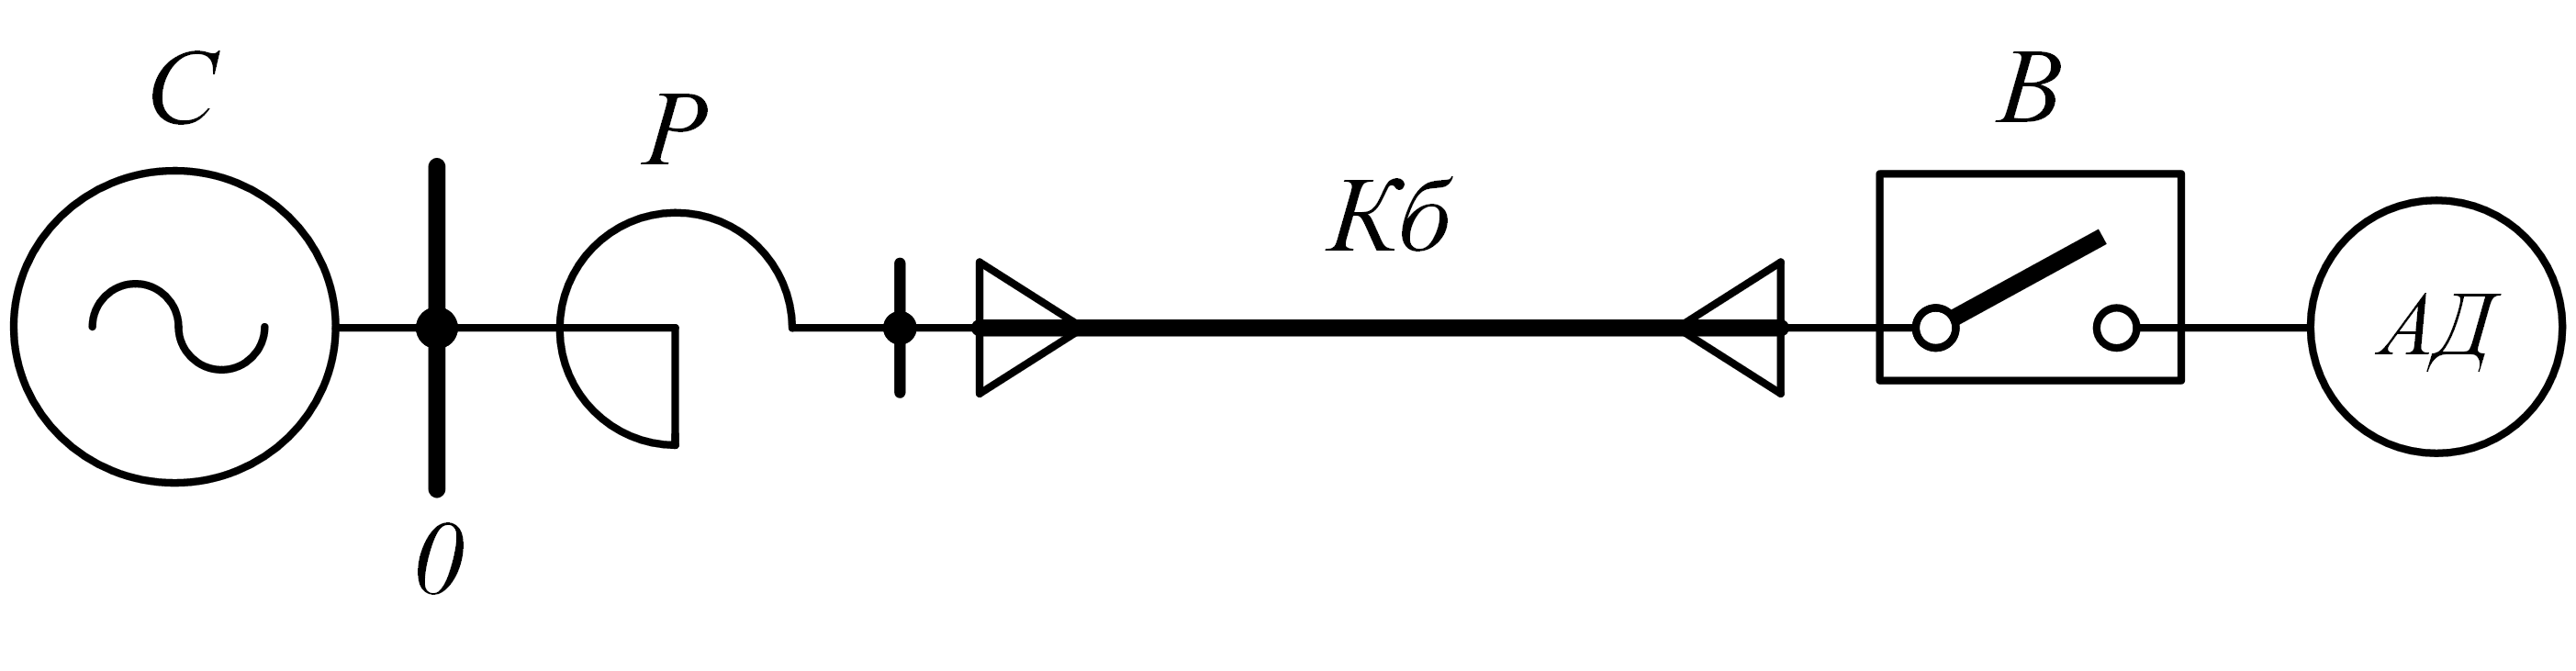
\includegraphics[width=0.5\linewidth]{pic/2-1}}
		\caption{Схема к примеру \ref*{chap:2 obshchie ukazaniia k vypolneniiu raschetov}-\arabic{example}.}
		\label{ris:example 2-1}
	\end{figure}
	
	Относительное базисные реактивности реактора и кабеля будут:

	\begin{equation*}
		{x_{\text{р}} = \frac{3}{100} \cdot \frac{280}{400} \cdot \frac{10}{6} = 0,035} 
	\end{equation*}

	и

	\begin{equation*}
		{x_{\text{Кб}} = 0,071 \cdot 1,25 \cdot \frac{2,9}{6^2} = 0,007}.
	\end{equation*}

	Относительное базисное напряжение на шинах источника составляет:

	\begin{equation*}
		{\underset{*}{U} = \frac{6,3}{6} = 1,05}.
	\end{equation*}
	
	Искомая величина пускового тока будет:
	
	\begin{equation*}
		{\underset{*}{I}\!\,_{\text{пуск}} = \frac{1,05}{0,035 + 0,007 + 0,18} = 4,74}.
	\end{equation*}
	
	Для определения пускового момента предварительно находим напряжение у двигателя при пуске:
	
	\begin{equation*}
		{\underset{*}{U} = 4,74 \cdot 0,18 = 0,85};
	\end{equation*}	
	
	следовательно, искомый пусковой момент составляет:
	
	\begin{equation*}
		{\underset{*}{M}\!\,_{\text{пуск}} = \underset{*}{U}^2 \underset{*}{M}\!\,_{\text{пуск.н}} = 0,85^2 \cdot 0,9 = 0,648}.
	\end{equation*}
\vspace{1pc}		
	
\end{small}

Выше рассмотрены величины, с которыми преимущественно приходится оперировать при выполнении обычных электрических расчетов. Однако, как отмечалось ранее, в системе относительных единиц можно выразить любые физические величины, в том числе и неэлектрические. Остановимся на определении относительных значений тех величин, с которыми придется иметь дело в дальнейшем.

За единицу измерения угловых скоростей обычно принимают синхронную угловую скорость $ \omega_{\text{с}} $  т.~е.  $ \omega_{\text{б}} = \omega_{\text{с}} $. Тогда произвольная угловая скорость в относительных базисных единицах будет:

\begin{equation} % 2-14
	\label{eq:2-14 omega_baz_otn}
	\underset{*}{\omega}\!\,_{\text{(б)}} = \frac{\omega}{\omega_{\text{б}}} = \frac{\omega}{\omega_{\text{с}}}.
\end{equation}

Соответственно этому в качестве базисных единиц принимают:\\
для индуктивности

\begin{equation*}
	L_{\text{б}} = \frac{z_{\text{б}}}{\omega_{\text{б}}} = \frac{z_{\text{б}}}{\omega_{\text{с}}};
\end{equation*}

для потокосцепления

\begin{equation*}
	\Psi_{\text{б}} = \frac{U_{\text{б}}}{\omega_{\text{б}}} = \frac{U_{\text{б}}}{\omega_{\text{с}}};
\end{equation*}

т.~е. потокосцепление, индуктирующее при базисной угловой скорости базисное напряжение.

Таким образом, при указанных базисных единицах и сохранении угловой скорости неизменной и равной синхронной, очевидно, имеем:

\begin{equation} % 2-15
	\label{eq:2-15 x_baz_otn_from_L}
	\underset{*}{x}\!\,_{\text{(б)}} = \underset{*}{\omega}\!\,_{\text{с}}\underset{*}{L}\!\,_{\text{(б)}} = \underset{*}{L}\!\,_{\text{(б)}};
\end{equation}

Вместо индуктивности $ L $ здесь может быть также взаимная индуктивность $ M $. % как бы это грамотно в footnote поместить?

\begin{equation} % 2-16
	\label{eq:2-16 Psi_baz_otn_from_I_and_L}
	\underset{*}{\Psi}\!\,_{\text{(б)}} = \underset{*}{I}\!\,_{\text{(б)}}\underset{*}{L}\!\,_{\text{(б)}} = \underset{*}{I}\!\,_{\text{(б)}}\underset{*}{x}\!\,_{\text{(б)}};
\end{equation}

\begin{equation} % 2-17
	\label{eq:2-17 E_baz_otn_from_omega_and_Psi}
	\underset{*}{E}\!\,_{\text{(б)}} = \underset{*}{\omega}\!\,_{\text{c}}\underset{*}{\Psi}\!\,_{\text{(б)}} = \underset{*}{\Psi}\!\,_{\text{(б)}};
\end{equation}

т.~е. при этих условиях индуктивное сопротивление численно равно индуктивности, а потокосцепление численно равно э.~д.~с. или соответствующему падению напряжения.

Подобная возможность замены одних относительных величин численно равными им другими представляет одно из существенных достоинств системы относительных единиц.

Время также можно выражать в относительных единицах. За единицу его измерения обычно принимают время, в течение которого ротор машины при синхронной скорости вращения повернется на один электрический радиан, т.~е. базисное время $ t_{\text{(б)}} = 1/\omega_{\text{с}} $, что при частоте 50~\textit{гц} составляет $ t_{\text{(б)}} = 1/314\text{~\textit{сек}} $. Следовательно, время, выраженное в относительных единицах, будет:

\begin{equation} % 2-18
	\label{eq:2-18 t_baz_otn}
	\underset{*}{t}\!\,_{\text{(б)}} = \frac{t}{t_{\text{(б)}}} = \omega_{\text{с}}t;
\end{equation}

при $ f = 50\text{~\textit{гц}} $

\begin{equation} % 2-18а
	\label{eq:2-18a t_baz_otn a}
	\underset{*}{t}\!\,_{\text{(б)}} = 314t.
	\tag{\ref*{eq:2-18 t_baz_otn}а}
\end{equation}

Для постоянной времени контура с $ L $ и $ r $ имеем:

\begin{equation*}
	T = \frac{L}{r} = \frac{x}{\omega_{\text{с}}r} = \frac{\underset{*}{x}\!\,_{\text{(б)}}}{\omega_{\text{с}}\underset{*}{r}\!\,_{\text{(б)}}},\text{~\textit{сек},}
\end{equation*}

чтобы перевести в относительные единицы, достаточно по (\ref{eq:2-18 t_baz_otn}) ее умножить на $ \omega_{\text{с}} $:

\begin{equation*}
	\underset{*}{T} = \omega_{\text{с}}T = \omega_{\text{с}}\frac{L}{r} = \frac{x}{r} = \frac{\underset{*}{x}\!\,_{\text{(б)}}}{\underset{*}{r}\!\,_{\text{(б)}}}.
\end{equation*}

Таким образом, относительная величина постоянной времени равна отношению индуктивного и активного сопротивлений, выраженных в именованных или относительных единицах.

Применение системы относительных единиц к цепям с магнитными связями, а также для роторных цепей электрических машин, где имеют место некоторые особенности, рассмотрено далее.

\section{Составление схемы замещения}
\label{sec:2-4 sostavlenie skhemy zameshcheniia}

При наличии трансформаторов (или автотрансформаторов) в схеме для упрощения проводимых расчетов такую схему целесообразно предварительно представить схемой замещения, т.~е. имеющиеся в ней магнитносвязанные цепи заменить одной эквивалентной электрически связанной цепью. Составление такой схемы замещения сводится к приведению параметров элементов и э.~д.~с. различных ступеней трансформации заданной схемы к какой-либо одной ступени, выбранной за основную. Само приведение осуществляется на основе соотношении, которые вытекают из известной теории трансформатора.

Чтобы исключить учет группы соединения обмоток трансформатора, в дальнейшем используем коэффициент трансформации, определяемый в соответствии с ранее принятым допущением (см.~§\ref{sec:2-1 osnovnye dopushcheniia}) как отношение междуфазных напряжений холостого хода его обмоток при установленных на них ответвлениях.

Пусть цепь некоторой ступени напряжения схемы связана с выбранной в этой схеме основной ступенью рядом каскадно включенных трансформаторов с коэффициентами трансформации $ k_1, k_2, \ldots k_n $. Используя известные соотношения для э.~д.~с. (напряжений), токов и сопротивлений при приведении их с одной стороны трансформатора на другую, можно записать общие выражения для определения приведенных к основной ступени значений отдельных величин этой цепи:

\begin{equation} % 2-19
	\label{eq:2-19 E_priveden_from_k}
	\overset{~\circ}{E} = (k_1, k_2, \ldots k_n)E;
\end{equation}

\begin{equation} % 2-19а
	\label{eq:2-19a U_priveden_from_k}
	\overset{\,\circ}{U} = (k_1, k_2, \ldots k_n)U;
	\tag{\ref*{eq:2-19 E_priveden_from_k}а}
\end{equation}

\begin{equation} % 2-20
	\label{eq:2-20 I_priveden_from_k}
	\overset{~\circ}{I} = \frac{1}{(k_1, k_2, \ldots k_n)}I;
\end{equation}

\begin{equation} % 2-21
	\label{eq:2-21 z_priveden_from_k}
	\overset{\,\circ}{z} = (k_1, k_2, \ldots k_n)^2z,
\end{equation}

% это должно быть в footnote
Кружок над буквой указывает, что данная величина является приведенной; для упрощения записи его часто опускают.

т.~е. истинные величины должны быть пересчитаны столько раз, сколько имеется трансформаторов на пути между приводимой цепью и принятой основной ступенью.

В этих и последующих выражениях под коэффициентом трансформации каждого трансформатора или автотрансформатора (как повышающего, так и понижающего) принимается \textit{отношение междуфазного напряжения холостого хода его обмотки, обращенной в сторону основной ступени напряжения, к аналогичному напряжению его другой обмотки, находящейся ближе к ступени, элементы которой подлежат приведению}.

Если величины заданы в относительных единицах, то их значения в именованных единицах определяют, исходя из соответствующих выражений §\ref{sec:2-3 sistema otnositelnykh edinitc}. Так, сопротивление элемента, для которого известно его $ \underset{*}{z}\!\,_{\text{(н)}} $, на основании (\ref{eq:2-8a z_nom_otn}) или (\ref{eq:2-9a z_nom_otn 2}) будет:

\begin{equation} % 2-22
	\label{eq:2-22 z_imen_from_nom_otn}
	z = \underset{*}{z}\!\,_{\text{(н)}}\frac{U_{\text{н}}}{\sqrt{3}I_{\text{н}}},\text{~\textit{ом}}
\end{equation}

или

\begin{equation} % 2-23
	\label{eq:2-23 z_imen_from_u_and_S}
	z = \underset{*}{z}\!\,_{\text{(н)}}\frac{U_{\text{н}}^2}{S_{\text{н}}},\text{~\textit{ом}}
\end{equation}

Рассмотренное приведение по действительным коэффициентам трансформации для сокращения называют точным приведением. В отличие от него в практических расчетах часто выполняют приближенное приведение, позволяющее значительно быстрее и проще получить приближенную схему замещения. Сущность такого приведения заключается в следующем.

Для каждой ступени трансформации устанавливают среднее номинальное напряжение $ U_{\text{ср}} $, а именно\footnote{Для ступеней ниже 1~\textit{кв} шкала средних номинальных напряжений приведена в \colorbox{red}{§ 17-5}.}:

\vspace{5pt}
\begin{center}
	\textbf{515; 340; 230; 154; 115; 37; 24; 20; 18; 15,75; 13,8; 10,5; 6,3; 3,15}~\textit{кв}
\end{center}
\vspace{5pt}

и при этом условно принимают, что номинальные напряжения всех элементов\footnote{Кроме реакторов, о чем указывалось в §\ref{sec:2-3 sistema otnositelnykh edinitc}.}, находящихся на одной ступени, одинаковы и равны соответствующим значениям по указанной шкале. Тогда коэффициент трансформации каждого трансформатора (или автотрансформатора), очевидно, равен отношению $ U_{\text{ср}} $ тех ступеней, которые он связывает, а результирующий коэффициент трансформации каскада трансформаторов будет определяться как отношение $ U_{\text{ср}} $ крайних ступеней. Следовательно, при приближенном приведении выражения для пересчета принимают более простой вид:

\begin{equation} % 2-24
	\label{eq:2-24 E_priveden_U_sred_and_U_baz}
	\overset{~\circ}{E} = \frac{U_{\text{ср.б}}}{U_{\text{ср}}}E;
\end{equation}

\begin{equation} % 2-24а
	\label{eq:2-24a U_priveden_U_sred_and_U_baz}
	\overset{\,\circ}{U} = \frac{U_{\text{ср.б}}}{U_{\text{ср}}}U; \tag{\ref*{eq:2-24 E_priveden_U_sred_and_U_baz}а}
\end{equation}

\begin{equation} % 2-25
	\label{eq:2-25 I_priveden_U_sred_and_U_baz}
	\overset{~\circ}{I} = \frac{U_{\text{ср.б}}}{U_{\text{ср}}}I;
\end{equation}

\begin{equation} % 2-26
	\label{eq:2-26 z_priveden_U_sred_and_U_baz}
	\overset{\,\circ}{z} = \left ( \frac{U_{\text{ср.б}}}{U_{\text{ср}}} \right )^{\!2}z,
\end{equation}

\begin{wrapfigure}[22]{l}{0.45\linewidth} % 2-2
	\centering
	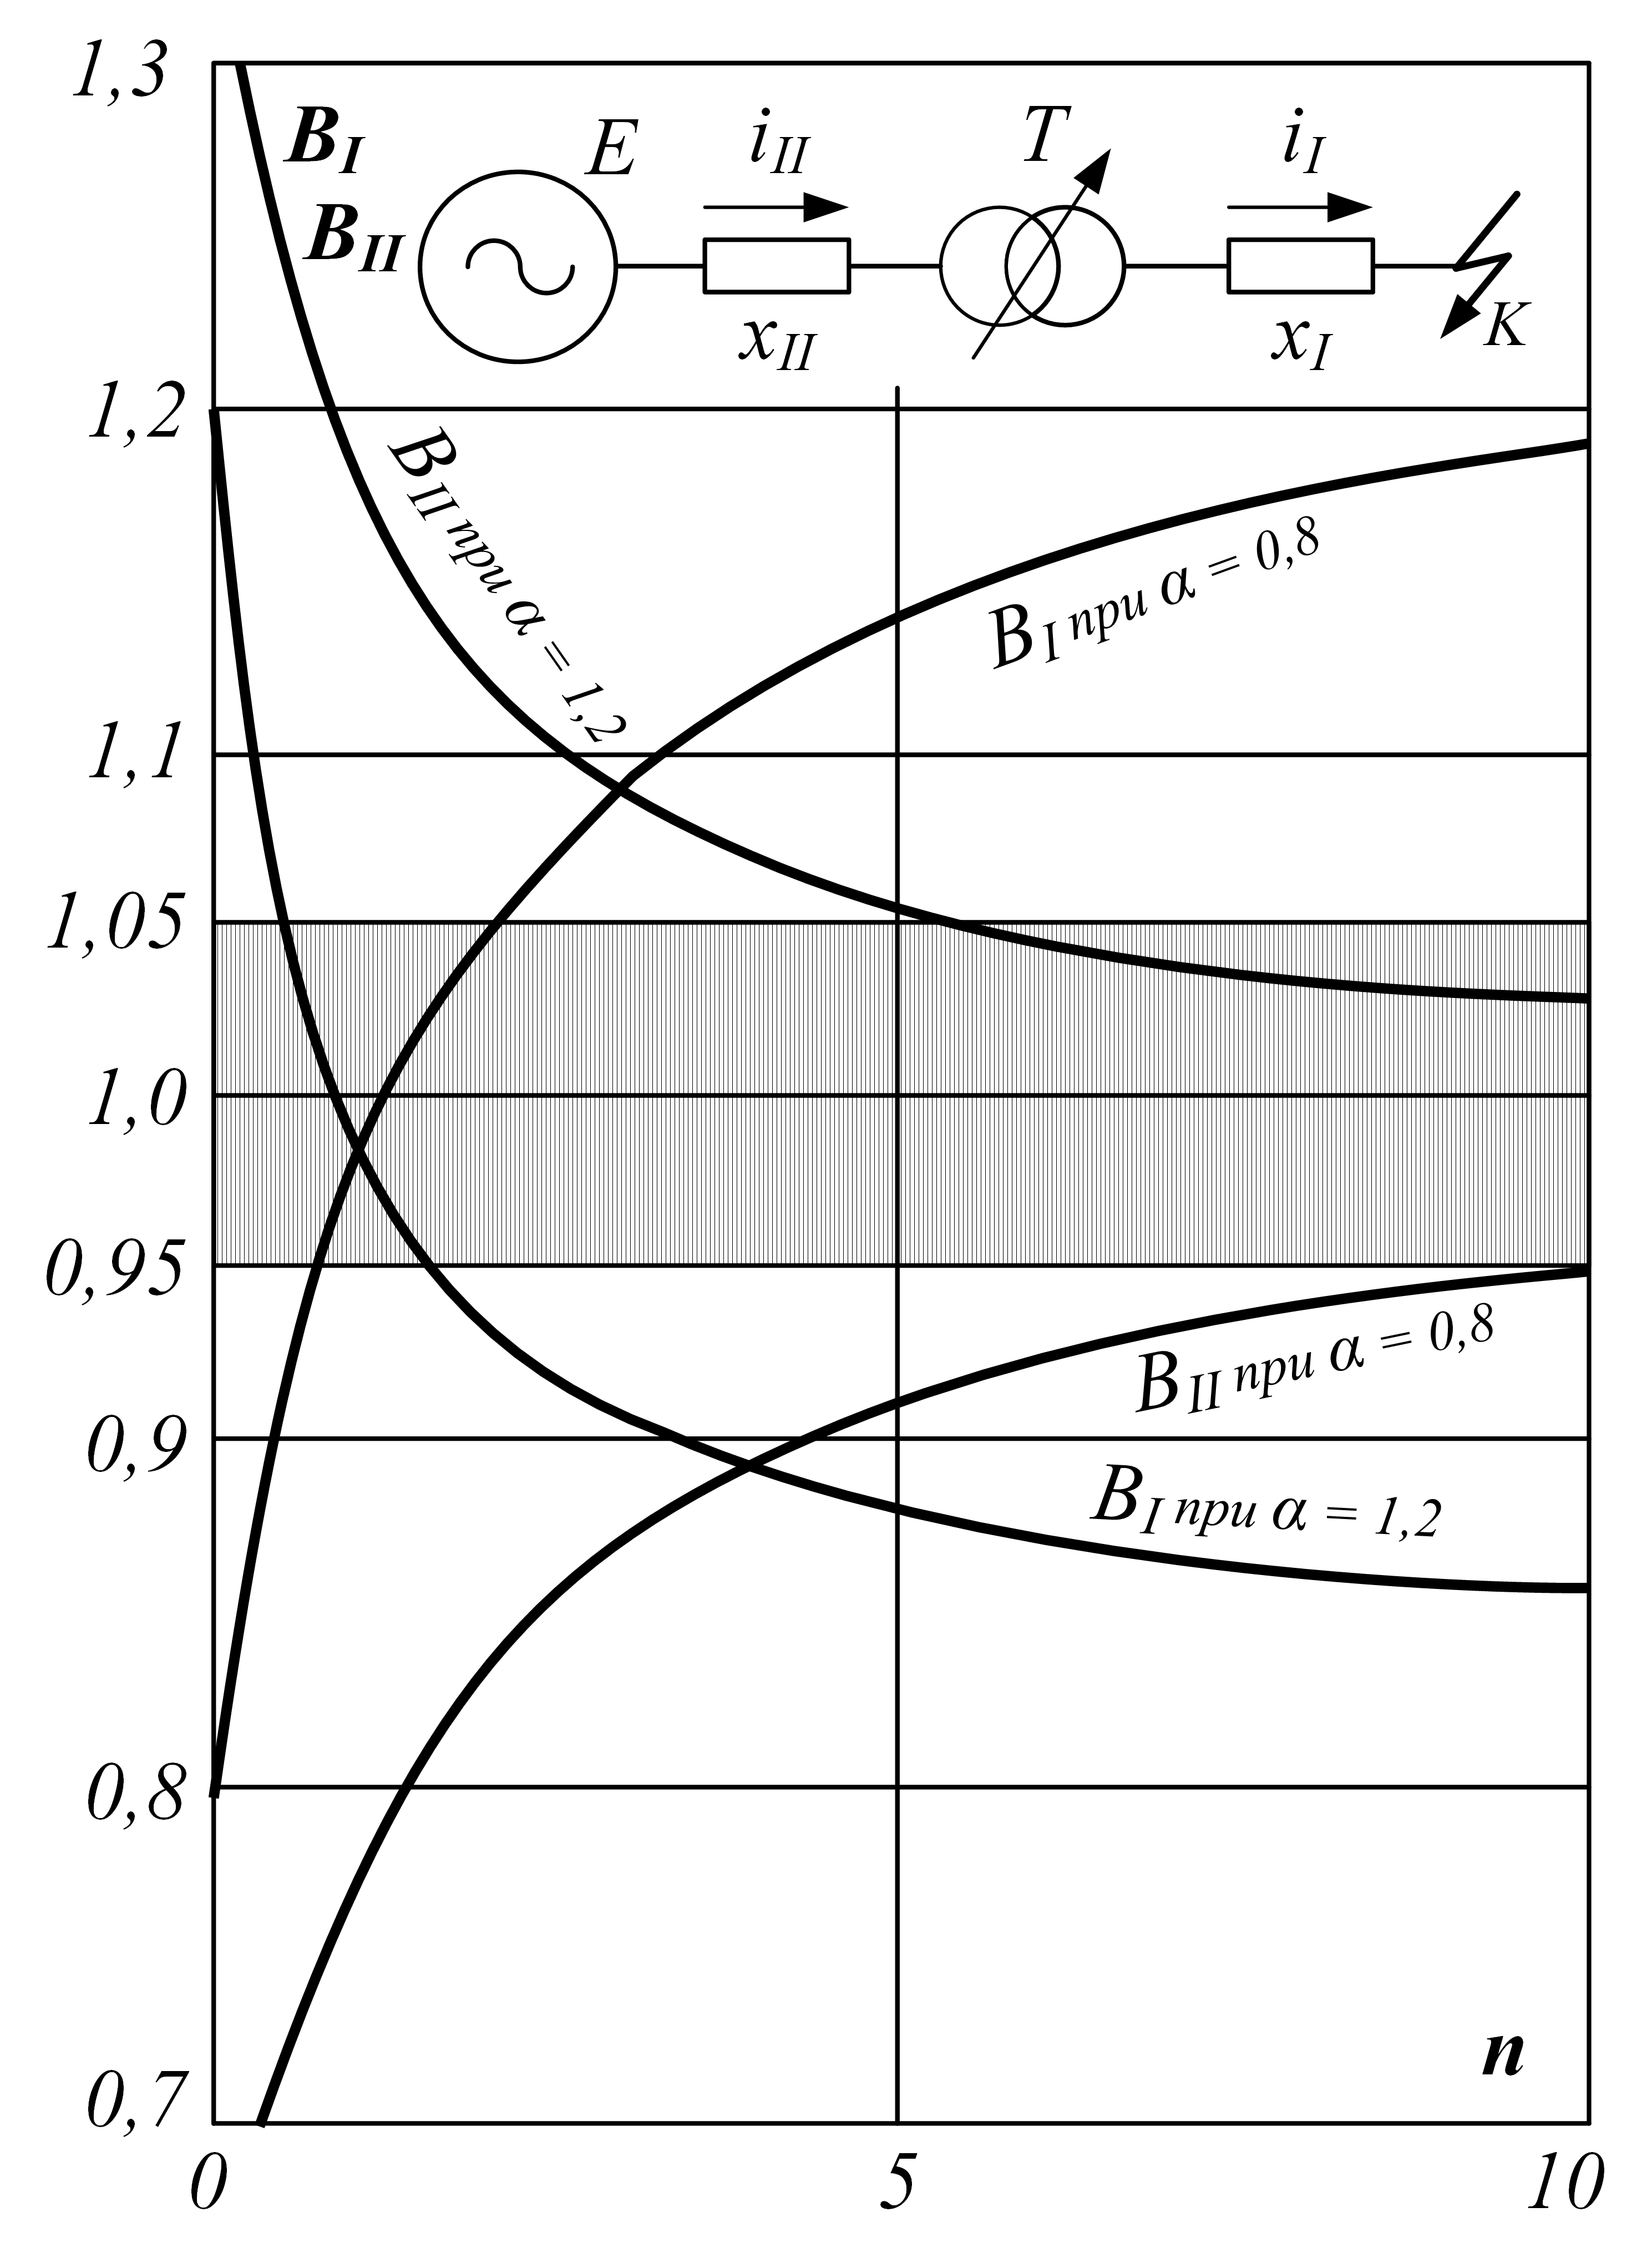
\includegraphics[width=0.95\linewidth]{pic/2-2}
	\caption{Кривые изменения отношений $ B_I $ и $ B_{II} $ в функциях $ n $.}
	\label{ris:2-2 B_I and B_I}
\end{wrapfigure}

где $ U_{\text{ср}} $ --- среднее номинальное напряжение ступени, с которой производится пересчет;\\
$ U_{\text{ср.б}} $ --- тоже выбранной основной степени.

Если элемент задан своим относительным сопротивлением $ \underset{*}{z}\!\,_{\text{(н)}} $, то его сопротивление в именованных единицах, приближенно приведенное к принятой основной ступени, легко определить по (\ref{eq:2-23 z_imen_from_u_and_S}), вводя в последнее вместо $ U_{\text{н}} $ среднее номинальное напряжение основной ступени.

Приближенное приведение схемы вносит некоторую погрешность в расчет; поэтому его надо применять с известной осторожностью. Для получения более надежных результатов приведение схемы следует производить по действительным коэффициентам трансформации, особенно в тех случаях, когда имеются трансформаторы (или автотрансформаторы) с широким диапазоном регулирования напряжения под нагрузкой (с РПН)\footnote{Так, например, по ГОСТ 12965-67 трехфазные двух- и трех- обмоточные трансформаторы с РПН мощностью 6,3~\textit{Мва} и выше должны иметь в нейтрали обмотки высшего напряжения регулирование $ \pm16\% $.} или специальные регулирующие устройства, как-то: линейные регулировочные автотрансформаторы (ЛРА), вольтодобавочные регулировочные трансформаторы (ВРТ).

\begin{small}
	\vspace{1pc}
	Чтобы иметь представление о порядке погрешности приближенного приведения, проведем исследование применительно к элементарной схеме, показанной в верхней части \colorbox{red}{рис. 2-2}, где для упрощения выкладок введены чисто индуктивные сопротивления $ x_I $ и $ x_{II} $. Ограничим свою задачу рассмотрением погрешностей только в токах при трехфазном коротком замыкании в точке $ K $.
	
	Если $ U_{\text{нI}} $ и $ U_{\text{нII}} $ --- номинальные напряжения обмоток трансформатора $ Т $, то при изменении числа витков обмотки $ I $ напряжение холостого хода будет $ U_I = \alpha U_{\text{нI}} $ и коэффициент трансформации $ k'=\alpha k $, где $ \alpha $ --- относительное отклонение указанного напряжения или коэффициента трансформации от их номинальных значений.
	
	В соответствии с принятым допущением (см.~§\ref{sec:2-3 sistema otnositelnykh edinitc}) при изменении числа витков регулируемой обмотки индуктивное сопротивление рассеяния трансформатора в делом, приведенное к стороне его нерегулируемой обмотки, остается постоянным. Поэтому в данном случае можно можно сказать, что оно включено в $ x_{II} $.
	
	При трехфазном коротком замыкании за $ x_I $ для токов имеем:
	
	\begin{equation} % 2-27
		\label{eq:2-27 I_I_tok_pri_kz_za_xI}
		I_I = \frac{\alpha k E}{x_I + \alpha^2 k^2 x_{II}}
	\end{equation}
	
	и
	
	\begin{equation} % 2-28
		\label{eq:2-28 I_II_tok_pri_kz_za_xI}
		I_{II} = \alpha k I_I.
	\end{equation}
	
	Найдем отношения значений этих токов при произвольном $ \alpha $ к их значениям при $ \alpha = 1 $. После небольших преобразований эти отношения можно представить в следующем виде:
	
	\begin{equation} % 2-29
		\label{eq:2-29 B_I_otnoshenie_tokov}
		B_I = \frac{I_I}{I_{I~(\alpha=1)}} = \frac{\alpha(1+n)}{1+\alpha^2 n};
	\end{equation}
	
	\begin{equation} % 2-30
		\label{eq:2-30 B_II_otnoshenie_tokov}
		B_{II} = \frac{I_{II}}{I_{II~(\alpha=1)}} = \alpha B_I,
	\end{equation}

	где $ n = \frac{k^2 x_{II}}{x_I} = \frac{\overset{\,\bullet}{x}_{II}}{x_I} = \frac{x_{II}}{\overset{\,\circ}{x}_I} $ --- отношение соответствующих реактивностей, приведенных к какой-либо одной ступени трансформации, при $ \alpha = 1 $.
	
	По этим выражениям при $ \alpha = 0,8 $ и $ \alpha = 1,2 $ построены кривые изменения $ B_I $ и $ B_{II} $ в функции $ n $ (рис.~\ref{ris:2-2 B_I and B_I}). Штриховкой отмечена зона отклонений $ B_I $ и $ B_{II} $ в пределах $ \pm 5 \% $; такая погрешность является вполне допустимой в большинстве практических расчетов токов короткого замыкания. Как видно, при указанном диапазоне отклонения $ \alpha $ погрешность приближенного решения может выходить достаточно далеко за пределы допустимой зоны. При заданном значении $ \alpha $ величины отношений $ B_I $ и $ B_{II} $ при изменении $ n $ от 0 до $ \infty $ находятся в пределах:
	
	\begin{equation*}
		B_I = \alpha \div \frac{1}{\alpha} \text{\quad и \quad} B_{II} = \alpha^2 \div 1,
	\end{equation*}
	
	причем если при $ \alpha \gtrless 1 $ всегда $ B_{II} \gtrless 1 $, то $ B_I $ в зависимости от $ n $ может быть как больше, так и меньше единицы. При малых значениях тока $ n $ погрешность приближенного определения тока $ I_{II} $ больше, чем тока $ I_I $, а при б\'{о}льших $ n $ имеет место обратное соотношение.
	
	Если в схеме рис.~\ref{ris:2-2 B_I and B_I} регулирование осуществляется на обмотке $ II $ (в данном случае на стороне источника), то коэффициент трансформации $ k' = U_{нI} / \beta U_{нII} = k / \beta $. Приняв $ \beta = 1/\alpha $, можно величины $ B_I $ и $ B_{II} $ определять по (\ref{eq:2-29 B_I_otnoshenie_tokov}) и (\ref{eq:2-30 B_II_otnoshenie_tokov}), где только при подсчете $ n $ реактивность трансформатора должна быть включена в $ x_I $, т.~е. в реактивность ступени $ I $.
	
	При каскаде трансформаторов ошибка приближенного приведения может как нарастать, так и, напротив, снижаться. Это зависит от установки регулируемых обмоток трансформаторов. Заранее
	предвидеть порядок этих погрешностей в общем случае невозможно.
	
	\vspace{1pc}
\end{small}

Используемые приближенные (без учета намагничивающего тока) схемы замещения трансформаторов и автотрансформаторов с двумя и б\'{о}льшим числом обмоток, а также с обмотками, расщепленными на параллельные ветви, приведены в приложении \colorbox{red}{П-7}, где также даны их некоторые типовые параметры. Линейные регулировочные автотрансформаторы следует рассматривать как обычные автотрансформаторы с переменным коэффициентом трансформации.

До сих нор предполагалось, что сопротивления элементов схемы замещения и э.~д.~с. определяются в именованных единицах. Разумеется, они могут быть выражены и в относительных единицах. Для этого, выбрав на основной ступени напряжения базисные условия, следует выполнить соответствующий пересчет.

Так, если сопротивление $ z $ связано с основной ступенью, для которой выбраны базисные величины $ U_{\text{б}} $ и $ I_{\text{б}} $ (или $ S_{\text{б}} $), трансформаторами с коэффициентами трансформации $ k_1, k_2, \ldots, k_n $, то в соответствии с (\ref{eq:2-21 z_priveden_from_k}) и (\ref{eq:2-8 z_baz_otn 2}) или (\ref{eq:2-9 z_baz_otn 3}) его относительная величина в схеме замещения будет:

\begin{equation} % 2-8б
	\label{eq:2-8b z_priveden_k_and_I_U}
	\underset{*}{z}\!\,_{\text{(б)}} = z(k_1 k_2, \ldots, k_n)^2 \frac{\sqrt{3} I_{\text{б}}}{U_{\text{б}}},
	\tag{\ref*{eq:2-8 z_baz_otn 2}б}
\end{equation}

или

\begin{equation} % 2-9б
	\label{eq:2-9b z_priveden_k_and_S_U}
	\underset{*}{z}\!\,_{\text{(б)}} = z(k_1 k_2, \ldots, k_n)^2 \frac{S_{\text{б}}}{U^2_{\text{б}}}.
	\tag{\ref*{eq:2-9 z_baz_otn 3}б}
\end{equation}

Этим выражениям можно придать тот же вид, что и (\ref{eq:2-8 z_baz_otn 2}) и (\ref{eq:2-9 z_baz_otn 3}), введя коэффициенты трансформации в соответствующие базисные величины, т.~е.

\begin{equation} % 2-8в
	\label{eq:2-8v z_priveden_k_and_I_U}
	\underset{*}{z}\!\,_{\text{(б)}} = z \frac{\sqrt{3} \overset{\;\circ}{I}_{\text{б}}}{\overset{\;\circ}{U}_{\text{б}}},
	\tag{\ref*{eq:2-8 z_baz_otn 2}в}
\end{equation}

или

\begin{equation} % 2-9в
	\label{eq:2-9v z_priveden_k_and_S_U}
	\underset{*}{z}\!\,_{\text{(б)}} = z \frac{\overset{\;\circ}{S}_{\text{б}}}{\overset{\!~\circ}{U^2_{\text{б}}}},
	\tag{\ref*{eq:2-8 z_baz_otn 2}в}
\end{equation}

где

\begin{equation} % 2-31
	\label{eq:2-31 U_baz_priv_k}
	\overset{\!\circ}{U^2_{\text{б}}} = \frac{1}{k_1 k_2, \ldots, k_n} U_{\text{б}},
\end{equation}

\begin{equation} % 2-32
	\label{eq:2-32 I_baz_priv_k}
	\overset{\circ}{I_{\text{б}}} = (k_1 k_2, \ldots, k_n) I_{\text{б}}
\end{equation}

или, иначе,

\begin{equation} % 2-32
	\label{eq:2-32a I_baz_priv_k 2}
	\overset{\circ}{I_{\text{б}}} = \frac{S_{\text{б}}}{\sqrt{3} \overset{\!\circ}{U_{\text{б}}}}.
	\tag{\ref*{eq:2-32 I_baz_priv_k}а}
\end{equation}

--- соответственно базисные напряжение и ток на той ступени, где находится данное сопротивление $ z $.

Следовательно, для составления эквивалентной схемы замещения в относительных единицах нужно прежде всего на одной из ступеней напряжения заданной схемы выбрать базисные единицы и затем по (\ref{eq:2-31 U_baz_priv_k}) --- (\ref{eq:2-32a I_baz_priv_k 2}) определить базисные единицы для каждой другой ступени напряжения. После этого по (\ref{eq:2-3 E_baz_otn}) --- (\ref{eq:2-5 I_baz_otn}), (\ref{eq:2-8 z_baz_otn 2}), (\ref{eq:2-9 z_baz_otn 3}) и (\ref{eq:2-11 E_baz_from_E_nom}) --- (\ref{eq:2-13 z_baz_from_z_nom 2}) следует подсчитать все величины в относительных единицах при базисных условиях, имея ввиду, что в каждом из указанных выражений под $ U_{\text{б}} $, $ I_{\text{б}} $ и $ z_{\text{б}} $ всегда надо понимать базисные напряжение, ток и сопротивление той ступени трансформации, на которой находятся подлежащие приведению величины.


При такой последовательности приведения магнитносвязанной схемы коэффициенты трансформации промежуточных трансформаторов (их определение -- см.~выше) учтены в базисных единицах каждой ступени напряжения заданной схемы.

Когда приведение схемы производится приближенно, пересчет к базисным условиям значительно упрощается, если за $ U_{\text{б}} $ принимать значение $ U_{\text{ср}} $ соответствующей ступени. В этом случае можно использовать (\ref{eq:2-8 z_baz_otn 2}) и (\ref{eq:2-9 z_baz_otn 3}), а также (\ref{eq:2-12a z_baz_from_z_nom a}) и (\ref{eq:2-13a z_baz_from_z_nom 2 a}), помня, что в (\ref{eq:2-12a z_baz_from_z_nom a}) $ I_{\text{б}} $ и $ I_{\text{н}} $ должны быть отнесены к одной ступени напряжения\footnote{Как отмечалось ранее, для реакторов пересчет по напряжениям
желателен, а в случае использования их в установках, напряжения которых меньше номинальных напряжений реакторов, --- обязателен.}.

Что касается э.~д.~с. и напряжений, то при этих условиях их относительные номинальные и базисные значения совпадают.

Следует особо подчеркнуть, что точность расчета, конечно, не зависит от того, в какой системе единиц выражены элементы эквивалентной схемы замещения. Последняя в обоих случаях, как показано выше, может быть составлена либо точно, либо приближений.

Магнитная связь в схеме возможна не только через трансформаторы или автотрансформаторы. Цепи одного или разных напряжений могут быть связаны взаимоиндукцией, влияние которой может сказываться весьма существенно. Наглядным примером служит сдвоенный реактор, где используется эффект взаимоиндукции между параллельными ветвями его обмотки. Схема замещения такого реактора и основные его характеристики приведены в приложении \colorbox{red}{П-5}. Очень сильно взаимоиндукция проявляется между воздушными линиями передачи, проходящими по общей трассе, при протекании по ним токов нулевой последовательности. В подобных случаях также целесообразно освободиться от магнитных связей, перейдя к соответствующей схеме замещения. Этот вопрос рассмотрен в \colorbox{red}{§12-7}, где приведены все необходимые указания.

Когда элементы схемы замещения выражены в именованных единицах, найденные в ней токи и напряжения являются реальными только для той ее части, ступень напряжения которой принята в качестве основной. Истинные токи и напряжения всех прочих участков схемы находят соответствующим пересчетом, исходя из (\ref{eq:2-19a U_priveden_from_k})) и (\ref{eq:2-20 I_priveden_from_k}) или (\ref{eq:2-24a U_priveden_U_sred_and_U_baz}) и (\ref{eq:2-25 I_priveden_U_sred_and_U_baz}). Если схема замещения составлена в системе относительных единиц, то для получения значений токов и напряжений в именованных единицах нужно найденные их относительные величины умножить на соответствующие базисные единицы данной ступени трансформации.

\addtocounter{example}{1}

\begin{small} % пример 2-2
	
	\vspace{1pc}
	\textit{Пример \ref*{chap:2 obshchie ukazaniia k vypolneniiu raschetov}-\arabic{example}}.
	Составить схему замещения для схемы рис.~\ref{ris:2-3 k_primeru},\textit{а,} выразив ее элементы в именованных и относительных единицах;	при этом сделать точное и приближенное приведение схемы.
	
	Вычислить начальные значения периодической слагающей тока при трехфазном коротком замыкании поочередно в точках \textit{K-1}, \textit{K-2} и \textit{K-3}.	Оценить влияние регулирования напряжения у трансформатора \textit{T-1} и линейного регулировочного автотрансформатора \textit{ЛРА} на величины указанных токов.
	
	\begin{figure}
		\begin{minipage}[h]{1\linewidth}
			\center{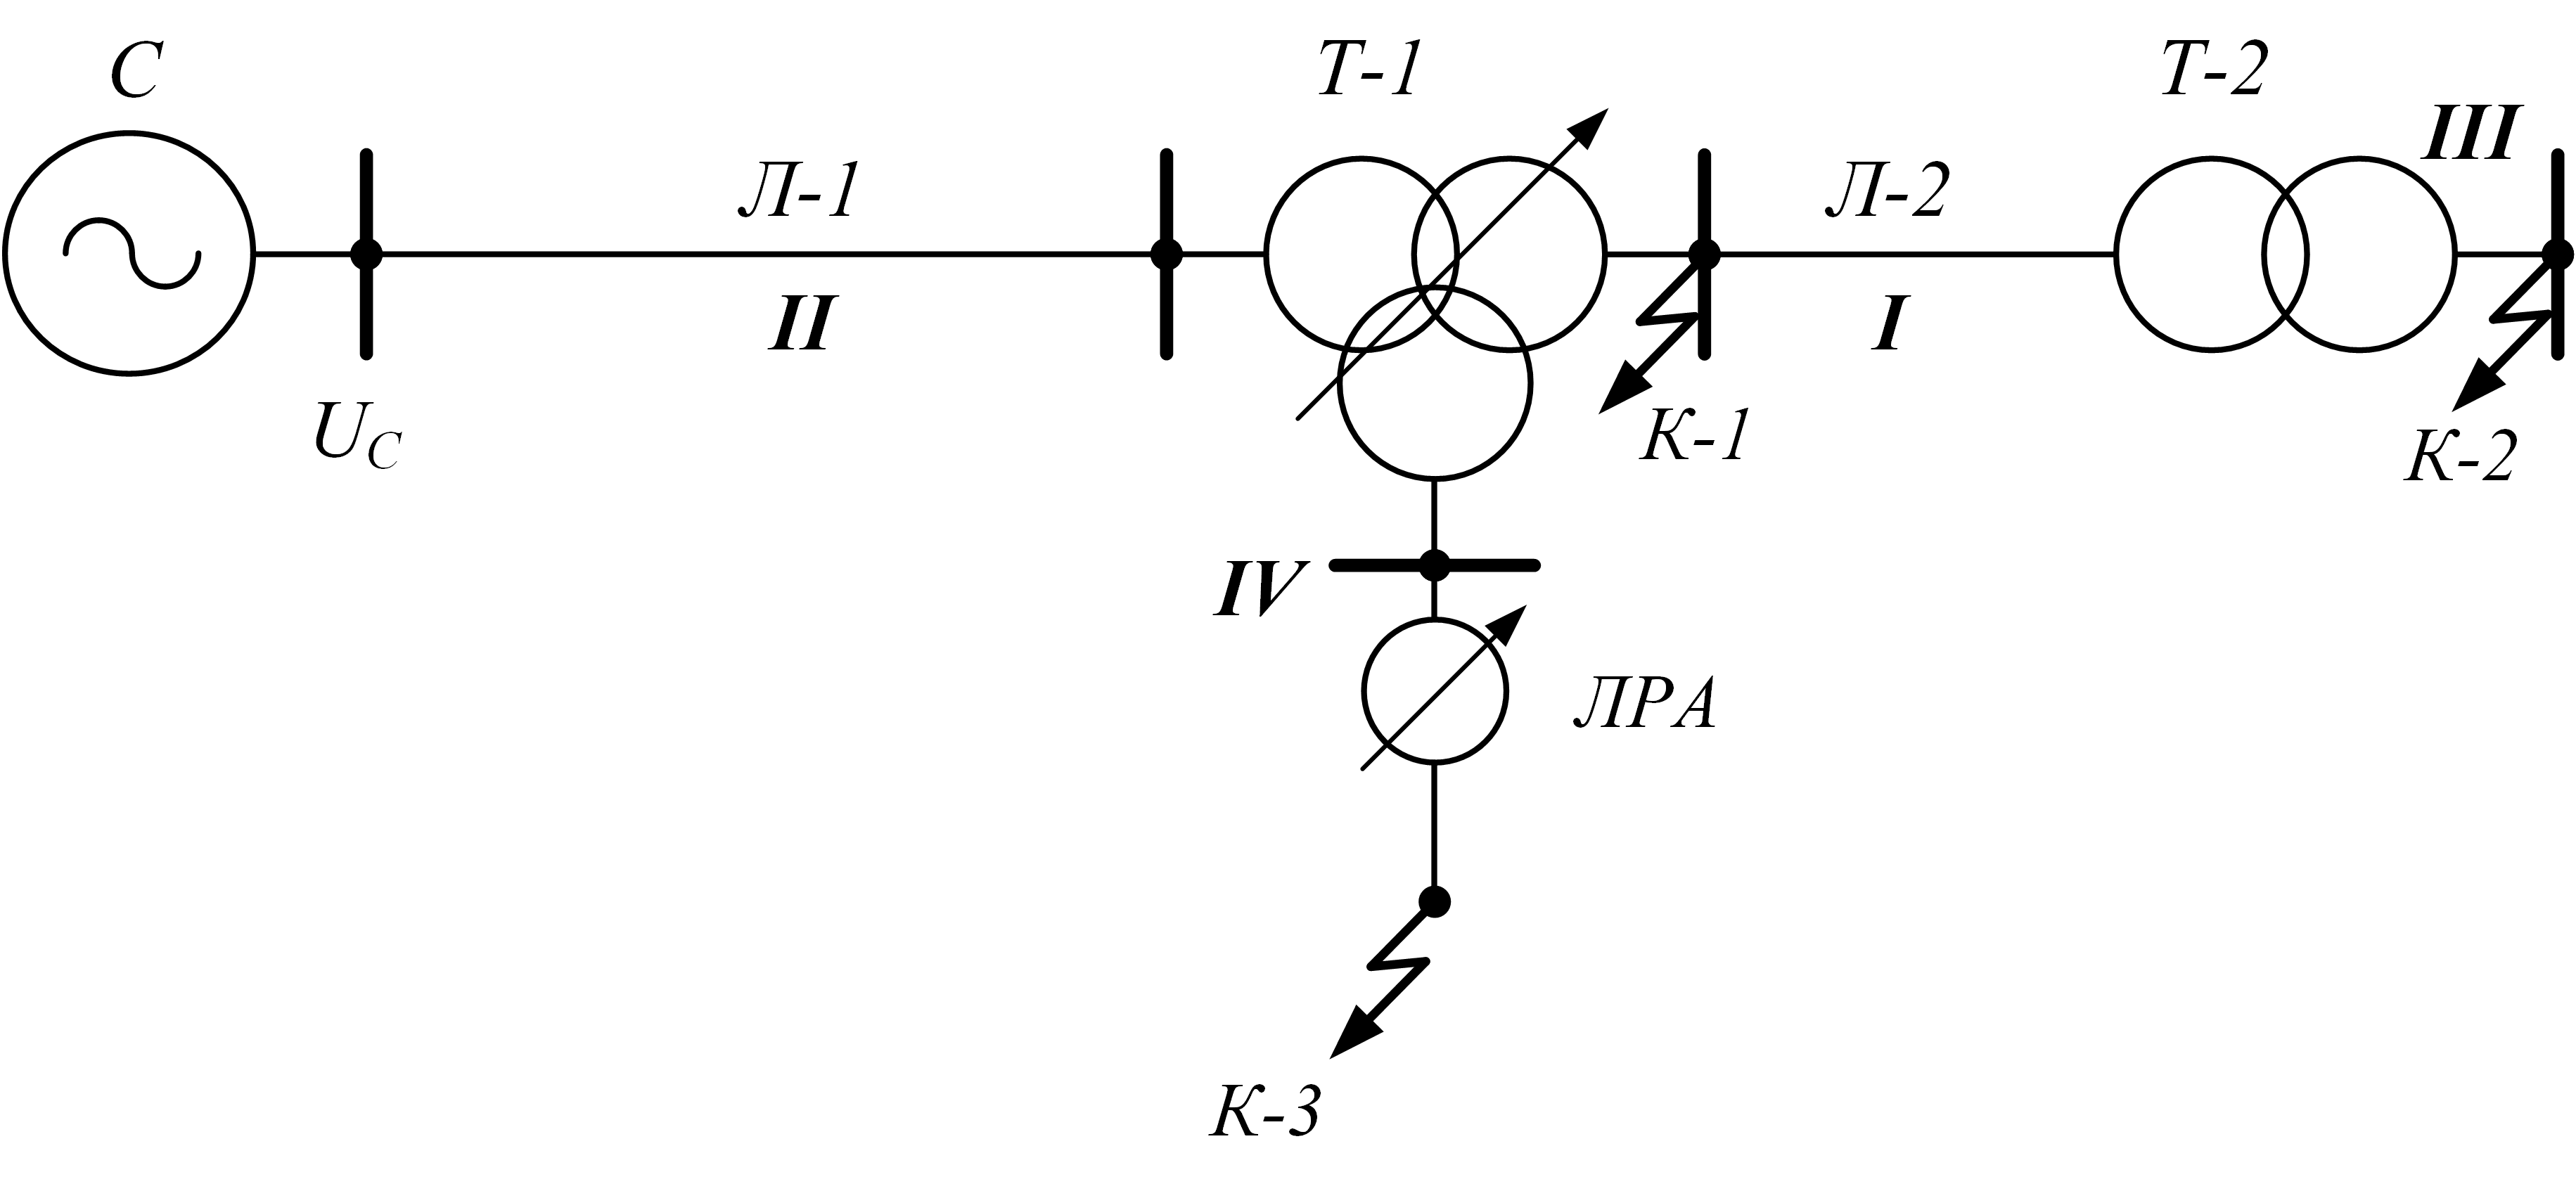
\includegraphics[width=0.6\linewidth]{pic/2-3_a} \\ \textit{а)}}
		\end{minipage}
		\vfill
		\begin{minipage}[h]{1\linewidth}
			\center{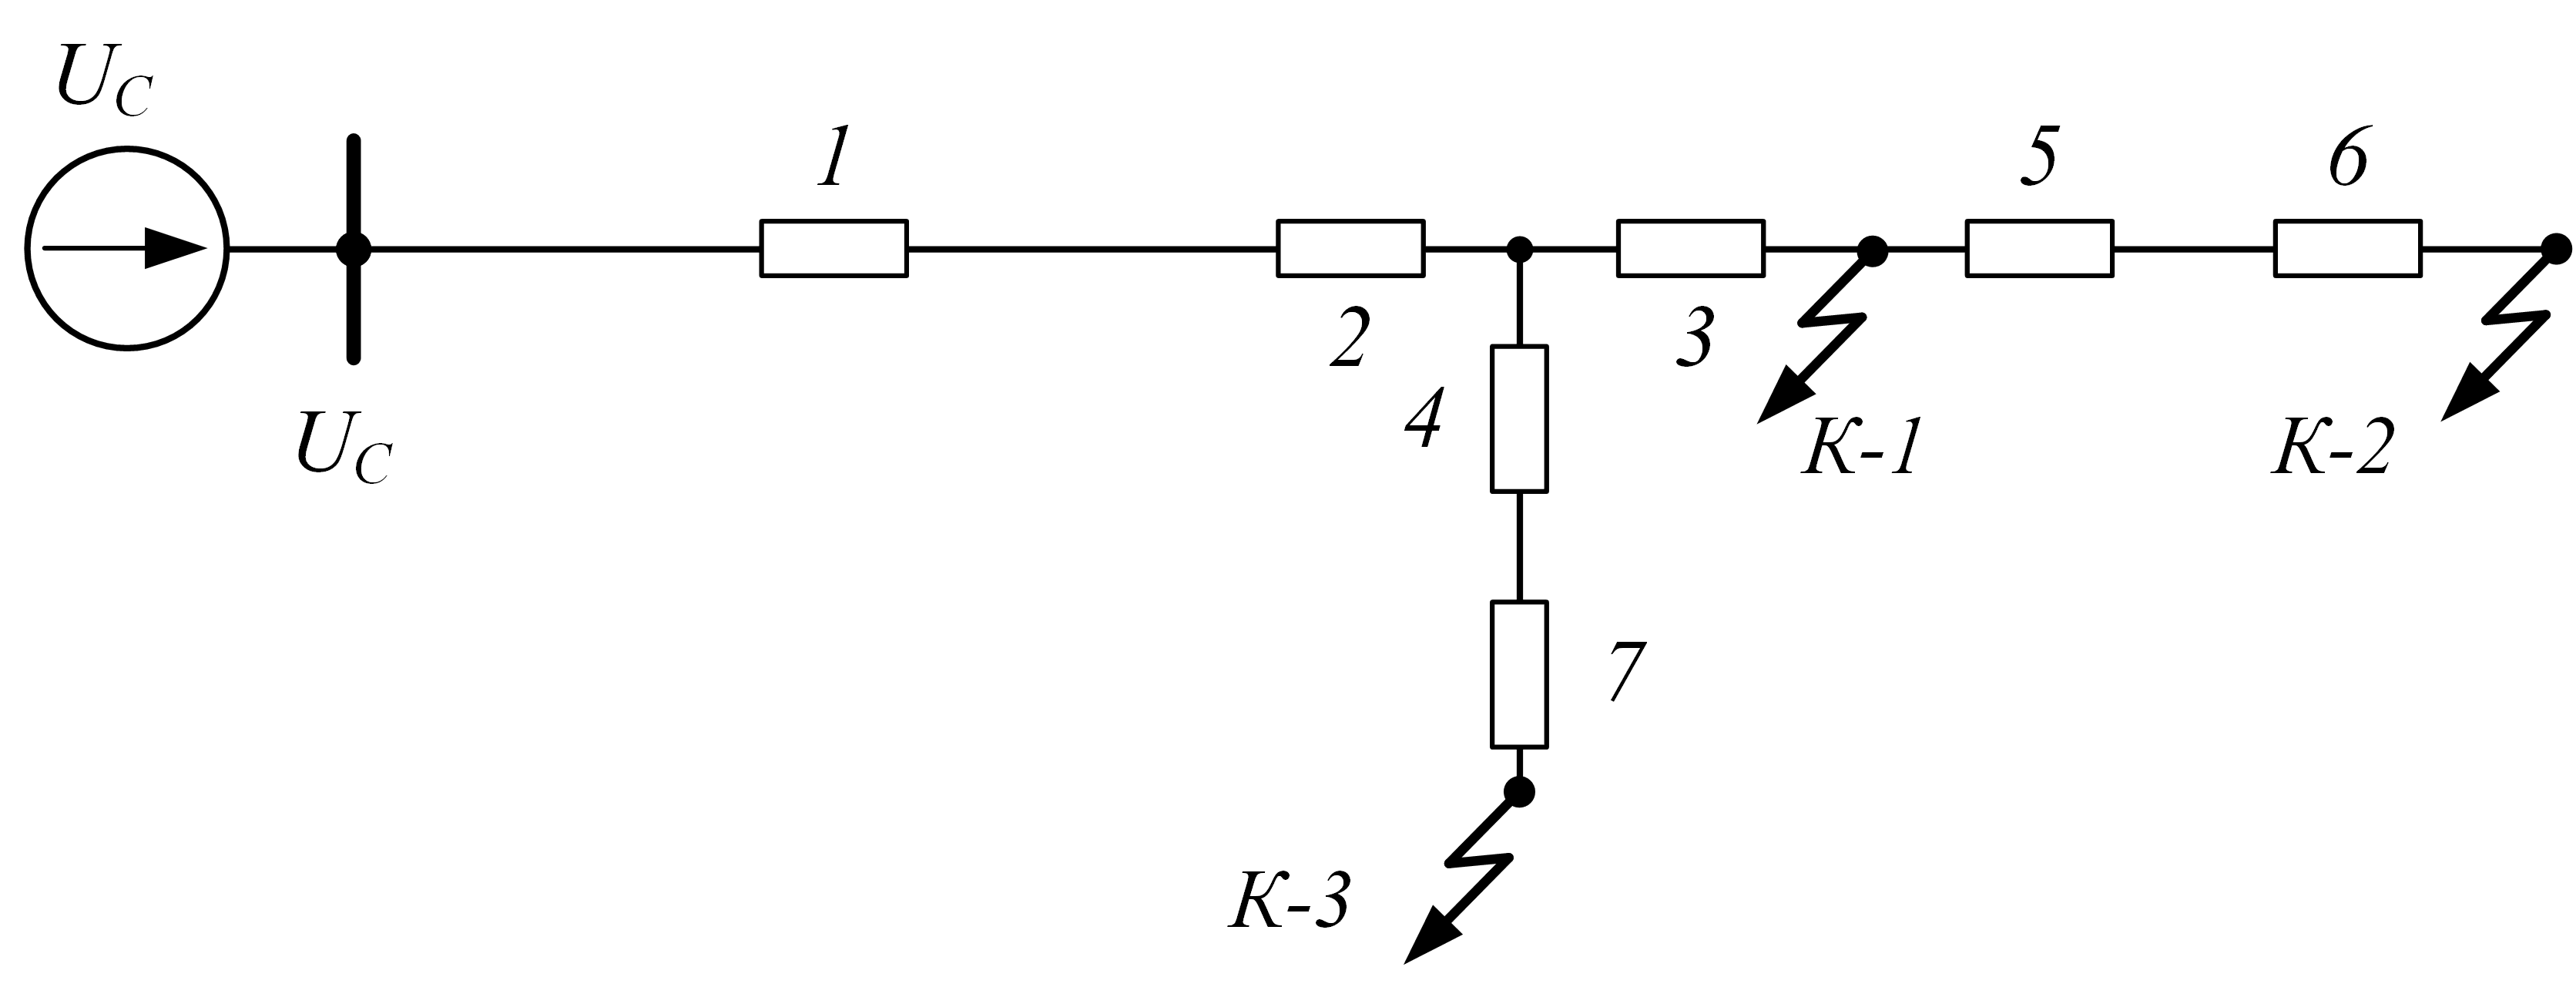
\includegraphics[width=0.6\linewidth]{pic/2-3_b} \\ \textit{б)}}
		\end{minipage}
		\caption{К примеру \ref*{chap:2 obshchie ukazaniia k vypolneniiu raschetov}-\arabic{example}. \textit{а} --- исходная схема; \textit{б} --- схема замещения.}
		\label{ris:2-3 k_primeru}
	\end{figure}
	
	Данные трансформатора \textit{Т-1} 40~\textit{Мва}, $ 115\pm16\% / 38,5 / 11$~\textit{кв}, $ u_{\text{ВС}} = 17\% $, $ u_{\text{ВН}} = 10,5\% $, $ u_{\text{СН}} = 6\% $;
	
	трансформатор \textit{Т-2} 6,3~\textit{Мва}, 35/6,6~\textit{кв}, $ u_K = 7,5\% $;
	
	линейный регулировочный трансформатор ЛРА 4~\textit{Мва}, 10~\textit{кв} $ \pm 10\% $, $ u_K = 0,5\% $;
	
	линия \textit{Л-1} 60~\textit{км}, x=0,4~ом/км;
	
	линия \textit{Л-2} 10~\textit{км}, x=0,4~ом/км;
	
	система \textit{С} --- напряжение практически неизменно и составляет $ U_{\text{С}} = 117 $~\textit{кв}.
	
	\vspace{1pc}
	\textit{а) Точное приведение в именованных единицах}
	
	В качестве основной выберем ступень, где включен источник.
	
	Схема замещения представленна на рис.~\ref{ris:2-3 k_primeru},\textit{б}. Реактивности ее элементов\footnote{Элементам схемы замещения рекомендуется давать порядковые номера, продолжая их для
		% В книжке опечатка "дли"
	элементов, которые получаются в результате производимого преобразования схемы.} будут:

	\begin{equation*}
		x_1 = 0,4 \cdot 60 = 24 \text{~\textit{ом}};
		\hspace{1pc}
		x_5 = 0.4 \cdot 10 \cdot \bigg(\frac{115}{38,5}\bigg)^2 = 36 \text{~\textit{ом}}.
	\end{equation*}

	Для \textit{Т-1} предварительно находим напряжения короткого замыкания каждой его обмотки (см.~\colorbox{red}{П-7}), т.~е. $ u_{\text{В}} = 0,5 (17 + 10,5 - 6 ) = 10,75 \% $; $ u_{\text{С}} = 17 - 10,75 = 6,25 \% $; $ u_{\text{Н}} = 6,0 - 6,25 = 0,25 \% $; следовательно, по (\ref{eq:2-23 z_imen_from_u_and_S})
	
	$ x_2 = \frac{10,75}{100} \cdot \frac{115^2}{40} = 35,5 \text{~ом} $; аналогично $ x_3 = 20,5 \text{~ом} $ и $ x_4 = -0,83 \text{~ом} $;
	
	для трансформатора \textit{Т-2}
	
	\begin{equation*}
		x_6 = \frac{7,5}{100} \cdot \frac{35^2}{6,3} \bigg(\frac{115}{38,5}\bigg)^2 = 131 \text{~\textit{ом}}.
	\end{equation*}
	
	и для ЛРА
	
	\begin{equation*}
		x_7 = \frac{0,5}{100} \cdot \frac{10^2}{4} \bigg(\frac{115}{11}\bigg)^2 = 13,6 \text{~\textit{ом}}.
	\end{equation*}
	
	Фазное напряжение источника
	
	\begin{equation*}
		U_{\text{С}} = \frac{117}{\sqrt{3}} = 67,5 \text{~\textit{кв}}.
	\end{equation*}
	
	Искомые величины токов составят:
	
	при коротком замыкании в \textit{К-1}
	
	ток в линии \textit{Л-1}
	
	\begin{equation*}
		I = \frac{67,5}{24 + 35,5 + 20,5} = \frac{67,5}{80} = 0,845 \text{~\textit{ка}};
	\end{equation*}
	
	в месте короткого замыкания
	
	\begin{equation*}
		I_{\text{К}} = 0,845 \cdot \frac{115}{38,5} = 2,53 \text{~\textit{ка}};
	\end{equation*}
	
	при коротком замыкании а \textit{К-2}
	
	ток в линии \textit{Л-1}
	
	\begin{equation*}
		I = \frac{67,5}{80 + 36 + 131} = \frac{67,5}{247} = 0,275 \text{~\textit{ка}};
	\end{equation*}
	
	в линии \textit{Л-2}
	
	\begin{equation*}
		I = 0,275 \cdot \frac{115}{38,5} = 0,82 \text{~\textit{ка}};
	\end{equation*}
	
	в месте короткого замыкания
	
	\begin{equation*}
		I_{\text{К}} = 0,82 \cdot \frac{35}{6,6} = 4,35 \text{~\textit{ка}};
	\end{equation*}
	
	при коротком замыкании в К-3 (без ЛРА)
	
	ток в линии \textit{Л-1}
	
	\begin{equation*}
		I = \frac{67,5}{24 + 35,5 + 0,83} = \frac{67,5}{58,8} = 1,17 \text{~\textit{ка}};
	\end{equation*}
	
	в месте короткого замыкания
	
	\begin{equation*}
		I_{\text{К}} = 1,17 \cdot \frac{115}{11} = 12,2 \text{~\textit{ка}}.
	\end{equation*}
	
	Произведем оценку влияния регулирования у \textit{Т-1} и \textit{ЛРА}.
	
	Пределы регулирования у \textit{Т-1} составляют $ \beta = 0,84 \div 1,16 $, чему соответствует $ \alpha = 1/\beta = 1/0,84 \div 1/1,16 = 1,19 \div 0,863 $. Теперь по (\ref{eq:2-29 B_I_otnoshenie_tokov}) и (\ref{eq:2-30 B_II_otnoshenie_tokov}) найдем значения искомых отклонений: при коротком замыкании в \textit{К-1} отношение $ n = \frac{24}{35,5 + 20,5} = 0,43 $, при котором отклонения в токе в месте короткого замыкания составляют от
	
	\begin{equation*}
		B_{\text{I}} = \frac{I_{\text{I}~(\alpha=0,863)}}{I_{\text{I}~(\alpha=1)}} = \frac{0,863 (1+0,43)}{1 + 0,863^2 \cdot 0,43} = 0,93
	\end{equation*}
	
	до
	
	\begin{equation*}
		B_\text{I} = \frac{I_{\text{I}~(\alpha=1,19)}}{I_{\text{I}~(\alpha=1)}} = \frac{1,19 (1+0,43)}{1 + 1,19^2 \cdot 0,43} = 1,06
	\end{equation*}
	
	и в токе линии \textit{Л-1}
	
	от $ B_{\text{II}} = 0,863 \cdot 0,93 = 0,8 $ до $ B_{\text{II}} = 1,19 \cdot 1,06 = 1,26 $.
	
	Аналогичный подсчет при коротком замыкании в \textit{К-2} дает для тока в месте короткого замыкания и в линии \textit{Л-2} $ B_{\text{I}} = 0,89 \div 1,14 $ и тока в линии \textit{Л-1} $ B_{\text{II}} = 0,77 \div 1,36 $; то же при коротком замыкании в \textit{К-3} для тока в месте короткого замыкания $ B_{\text{I}} = 0,95 \div 1,04 $ и тока в линии \textit{Л-1} $ B_{\text{II}} = 0,80 \div 1,24 $.
	
	В последнем случае, если дополнительно учесть регулирование на \textit{ЛРА} (введя, конечно, и его реактивность), величина тока в месте короткого замыкания может изменяться в пределах  8,3--11~\textit{ка}.
	
	\vspace{1pc}
	\textit{б) Приближенное приведение в именованных единицах}
	
	В соответствии с рекомендованной шкалой принимаем, что средние номинальное напряжение ступеней заданной схемы составляют: 110; 37; 10,5 и 6,3~\textit{кв}. В качестве основной сохраним ступень, где включен источник; при этом, очевидно, реактивности $ x_1 $, $ x_2 $, $ x_3 $ и $ x $ останутся теми же, а остальные будут:
	
	\begin{equation*}
		x_5 = 0,4 \cdot 10 \cdot \bigg( \frac{115}{37} \bigg)^2 = 38,7 \text{~\textit{ом}
		\hspace{1pc} и \hspace{1pc}}
		x_6 = \frac{7,5}{100} \cdot \frac{115^2}{6,3} = 157 \text{~\textit{ом}}
	\end{equation*}
	
	Величины токов при коротких замыканиях:
	
	в \textit{К-1}
	
	\begin{equation*}
		I_{\text{К}} = \frac{67,5}{24 + 35,5 + 20,5} \cdot \bigg( \frac{115}{37} \bigg) = 2,63 \text{~\textit{ка} (примерно больше на 4\%)};
	\end{equation*}
	
	в \textit{К-2}
	
	\begin{equation*}
		I_{\text{К}} = \frac{67,5}{80 + 38,7 + 157} \cdot \bigg( \frac{115}{6,3} \bigg) = 4,46 \text{~\textit{ка} (примерно больше на 2\%)};
	\end{equation*}
	
	в \textit{К-3}
	
	\begin{equation*}
		I_{\text{К}} = \frac{67,5}{24 + 35,5 - 0,83} \cdot \bigg( \frac{115}{10,5} \bigg) = 12,8 \text{~\textit{ка} (больше на 6,5\%)}.
	\end{equation*}
	
	\vspace{1pc}
	\textit{в) Точное приведение в относительных единицах}
	
	Примем $ S_{\text{б}} = 1000 $ ~\textit{Мва} и на ступени II $ U_{\text{бII}} = 115 $ ~\textit{кв}. Тогда $ I_{\text{бII}} = \frac{1000}{\sqrt{3} \cdot 115} = 5 $~\textit{ка} и на других ступенях базисные напряжения и токи будут:
	
	\begin{equation*}
		U_{\text{бI}} = 115 \cdot \frac{38,5}{115} = 38,5\text{~\textit{кв}};
		\hspace{1pc}
		I_{\text{бI}} = 5 \cdot \frac{115}{38,5} = 15\text{~\textit{ка}};
	\end{equation*}
	
	\begin{equation*}
		U_{\text{бIII}} = 38,5 \cdot \frac{6,6}{35} = 7,25\text{~\textit{кв}};
		\hspace{1pc}
		I_{\text{бIII}} = 15 \cdot \frac{35}{6,6} = 79,5\text{~\textit{ка}};
	\end{equation*}
	
	\begin{equation*}
		U_{\text{бIV}} = 115 \cdot \frac{11}{115} = 11\text{~\textit{кв}};
		\hspace{1pc}
		I_{\text{бIV}} = 5 \cdot \frac{115}{11} = 52,3\text{~\textit{ка}}.
	\end{equation*}
	
	Пользуясь соответствующими выражениями, находим:
	
	\begin{equation*}
		x_1 = 0,4 \cdot 60 \cdot \frac{1000}{115^2} = 1,82;
		\hspace{1pc}
		x_2 = 0,1075 \cdot \frac{1000}{40} = 2,69;
	\end{equation*}
	
	\begin{equation*}
		\text{аналогично} \hspace{1pc} x_3 = 1,56 \hspace{1pc}\text{и}\hspace{1pc} x_4 = -0,06; \hspace{1pc} x_5 = 0,4 \cdot 10 \cdot \frac{1000}{38,5^2} = 2,7;
	\end{equation*}
	
	\begin{equation*}
		\text{и\hspace{1pc}} x_6 = 0,075 \cdot \frac{1000}{6,3} \cdot \bigg( \frac{35}{38,5} \bigg)^2 = 9,83;
	\end{equation*}
	
	относительное напряжение источника
	
	\begin{equation*}
		U_{\text{С}} = \frac{117}{115} = 1,02.
	\end{equation*}
	
	При коротком замыкании а \textit{К-1} величина относительного тока будет:
	
	\begin{equation*}
		I = \frac{1,02}{1,82 + 2,69 + 1,56} = \frac{1,02}{6,07} = 0,169.
	\end{equation*}
	
	Значения токов на ступени соответствующего напряжения будут:
	
	в линии \textit{Л-1}
	
	\begin{equation*}
		I = 0,169 \cdot 5 = 0,845 \text{~\textit{ка}},
	\end{equation*}
	
	в месте короткого замыкания
	
	\begin{equation*}
		I_{\text{К}} = 0,169 \cdot 15 = 2,53 \text{~\textit{ка}}.
	\end{equation*}
	
	При коротком замыкании в \textit{К-2}
	
	\begin{equation*}
		\underset{*}{I} = \frac{1,02}{6,07 + 2,69 + 9,83} = \frac{1,02}{18,6} = 0,055;
	\end{equation*}
	
	ток в линии \textit{Л-1}
	
	\begin{equation*}
		I = 0,055 \cdot 5 = 0,275 \text{~\textit{ка}};
	\end{equation*}
		
	ток в линии \textit{Л-2}
	
	\begin{equation*}
		I = 0,055 \cdot 15 = 0,82 \text{~\textit{ка}};
	\end{equation*}
		
	в месте короткого замыкания
	
	\begin{equation*}
		I_{\text{К}} = 0,055 \cdot 79,5 = 4,35 \text{~\textit{ка}}.
	\end{equation*}
	
	При коротком замыкании в \textit{К-3}
	
	\begin{equation*}
		\underset{*}{I} = \frac{1,02}{1,82 + 2,69 - 0,06} = \frac{1,02}{4,45} = 0,23;
	\end{equation*}	
	
	ток в линии \textit{Л-1}
	
	\begin{equation*}
		I = 0,23 \cdot 5 = 1,15 \text{~\textit{ка}};
	\end{equation*}
	
	в месте короткого замыкания
	
	\begin{equation*}
		I_{\text{К}} = 0,23 \cdot 52,3 = 12 \text{~\textit{ка}}.
	\end{equation*}
	
	Все полученные величины токов, как и следовало ожидать, совпадают соответственно с теми, которые были найдены при точном решении в именованных единицах.
	
	Рекомендуется читателю самостоятельно убедиться в тождественности результатов приближенного определения токов в именованных и относительных единицах.
	
	Учет вольтодобавочного регулировочного трансформатора показан в решении примера \hyperref[exmpl:2-3]{2.3}.
	
\end{small}

\section{Преобразование схем замещения}
\label{sec:2-5 preobrazovanie_skhem_zameshcheniia}

В частном случае, когда схема замещения не содержит замкнутых контуров и в ней имеется один или несколько источников с одинаковыми э.~д.~с, ее можно легко привести к простейшему виду путем элементарных преобразований последовательного и параллельного сложения элементов). В общем же случае для такого приведения используют ряд дополнительных преобразований, как в обычных расчетах линейных электрических цепей. К ним относятся преобразования треугольника в звезду или обратно, многолучевой звезды в полный (с диагоналями) многоугольник, замена нескольких генерирующих ветвей с разными э.~д.~с, присоединенных к общему узлу, одной эквивалентной. Формулы таких преобразований для справки помещены в приложении \colorbox{red}{П-1}.

Приведем ряд указаний и рекомендаций, которыми следует руководствоваться при преобразовании схем в ходе выполнения расчетов, учитывая некоторые специфические особенности последних.

Первоочередной задачей расчета коротких замыкании обычно является нахождение тока непосредственно в аварийной ветви или в месте короткого замыкания. Поэтому преобразование схемы выгодно вести так, чтобы аварийная ветвь по возможности была сохранена до конца преобразования или в крайнем случае участвовала в нем только на последних его этапах. С этой целью, в частности, концы нагрузочных ветвей, э.~д.~с. которых принимаются равными нулю, не следует соединять с точкой трехфазного короткого замыкания, а лучше эти ветви объединять с генераторами в эквивалентные ветви.

Когда металлическое трехфазное короткое замыкание находится в узле с несколькими сходящимися в нем ветвями (рис.~\ref{ris:2-4 primer_preobrazovaniia_skhemy},\textit{а}), этот узел можно разрезать, сохранив на конце каждой образовавшейся ветви такое же короткое замыкание (рис.~\ref{ris:2-4 primer_preobrazovaniia_skhemy},\textit{б}). Далее полученную схему нетрудно преобразовать относительно любой из точек короткого замыкания, учитывая другие ветви с короткими замыканиями как обычные нагрузочные ветви с э.~д.~с, равными нулю. Такой прием особенно эффективен, когда нужно найти ток в одной иа ветвей, присоединенных к узлу короткого замыкания.

Довольно часто встречается симметрия схемы относительно точки короткого замыкания или симметрия какого-нибудь участка схемы относительно некоторой промежуточной точки. Использование этого обстоятельства позволяет значительно упростить преобразование схемы. Так, например, пусть в схеме рис.~\ref{ris:2-4 primer_preobrazovaniia_skhemy},\textit{а} элементы, расположенные симметрично относительно элемента \textit{7}, одинаковы. Тогда, очевидно, потенциалы узлов, где присоединены ветви \textit{1} и \textit{3}, также одинаковы, что позволяет эти узлы закоротить и образовавшиеся параллельные ветви \textit{1} и \textit{3}, \textit{4} и \textit{5}, \textit{6} и \textit{8} заменить эквивалентными. Вместо двух контуров схема теперь содержит один контур, преобразовав который в эквивалентную звезду, уже совеем легко привести схему к элементарному виду. Если в схеме рис.~\ref{ris:2-4 primer_preobrazovaniia_skhemy},\textit{а} генерирующие ветви \textit{1}, \textit{2} и \textit{3} одинаковы, а также одинаковы элементы \textit{6}, \textit{7} и \textit{5}, то наличие элементов \textit{4} и \textit{5} при рассматриваемом положении точки короткого замыкания никак не сказывается, т.~е. каждая генерирующая ветвь с соответствующим ей элементом (\textit{6}, \textit{7}, \textit{8}) является независимой.

\begin{figure}[]
	\begin{minipage}[h]{0.47\linewidth}
		\center{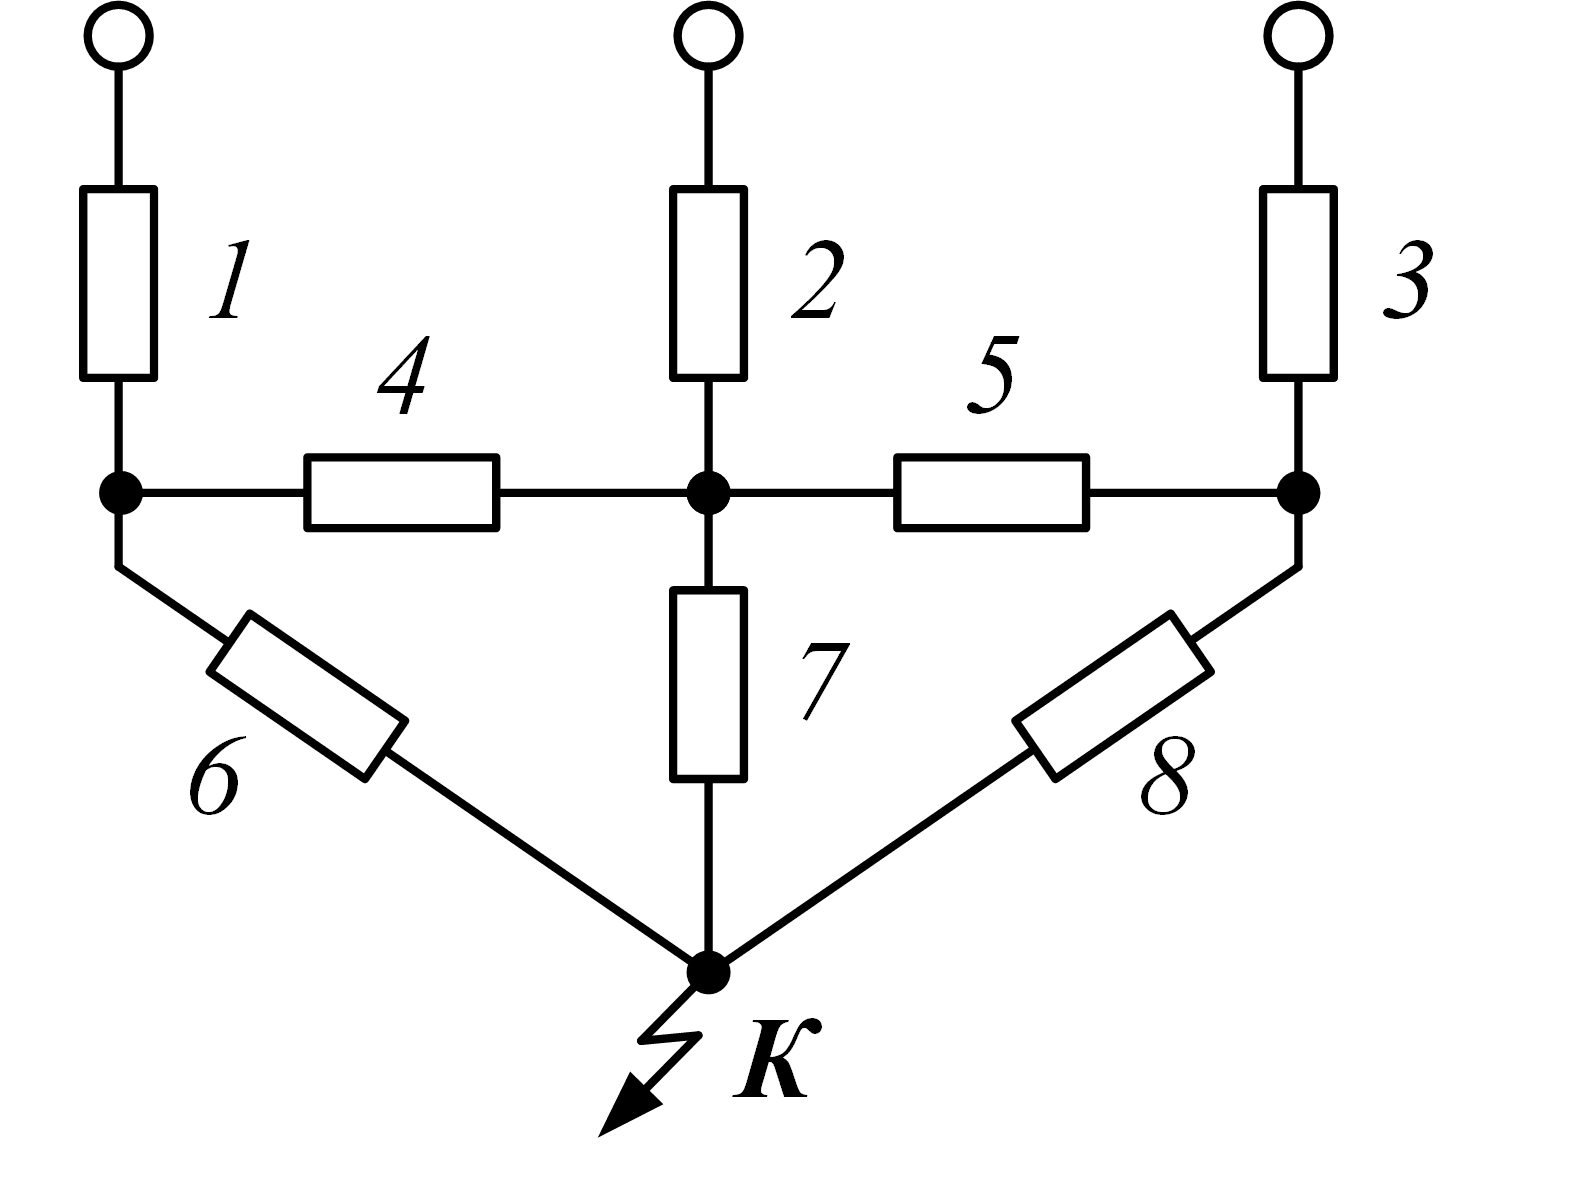
\includegraphics[width=1\linewidth]{pic/2-4_a}} \\ \textit{а)}
	\end{minipage}
	\hfill
	\begin{minipage}[h]{0.47\linewidth}
		\center{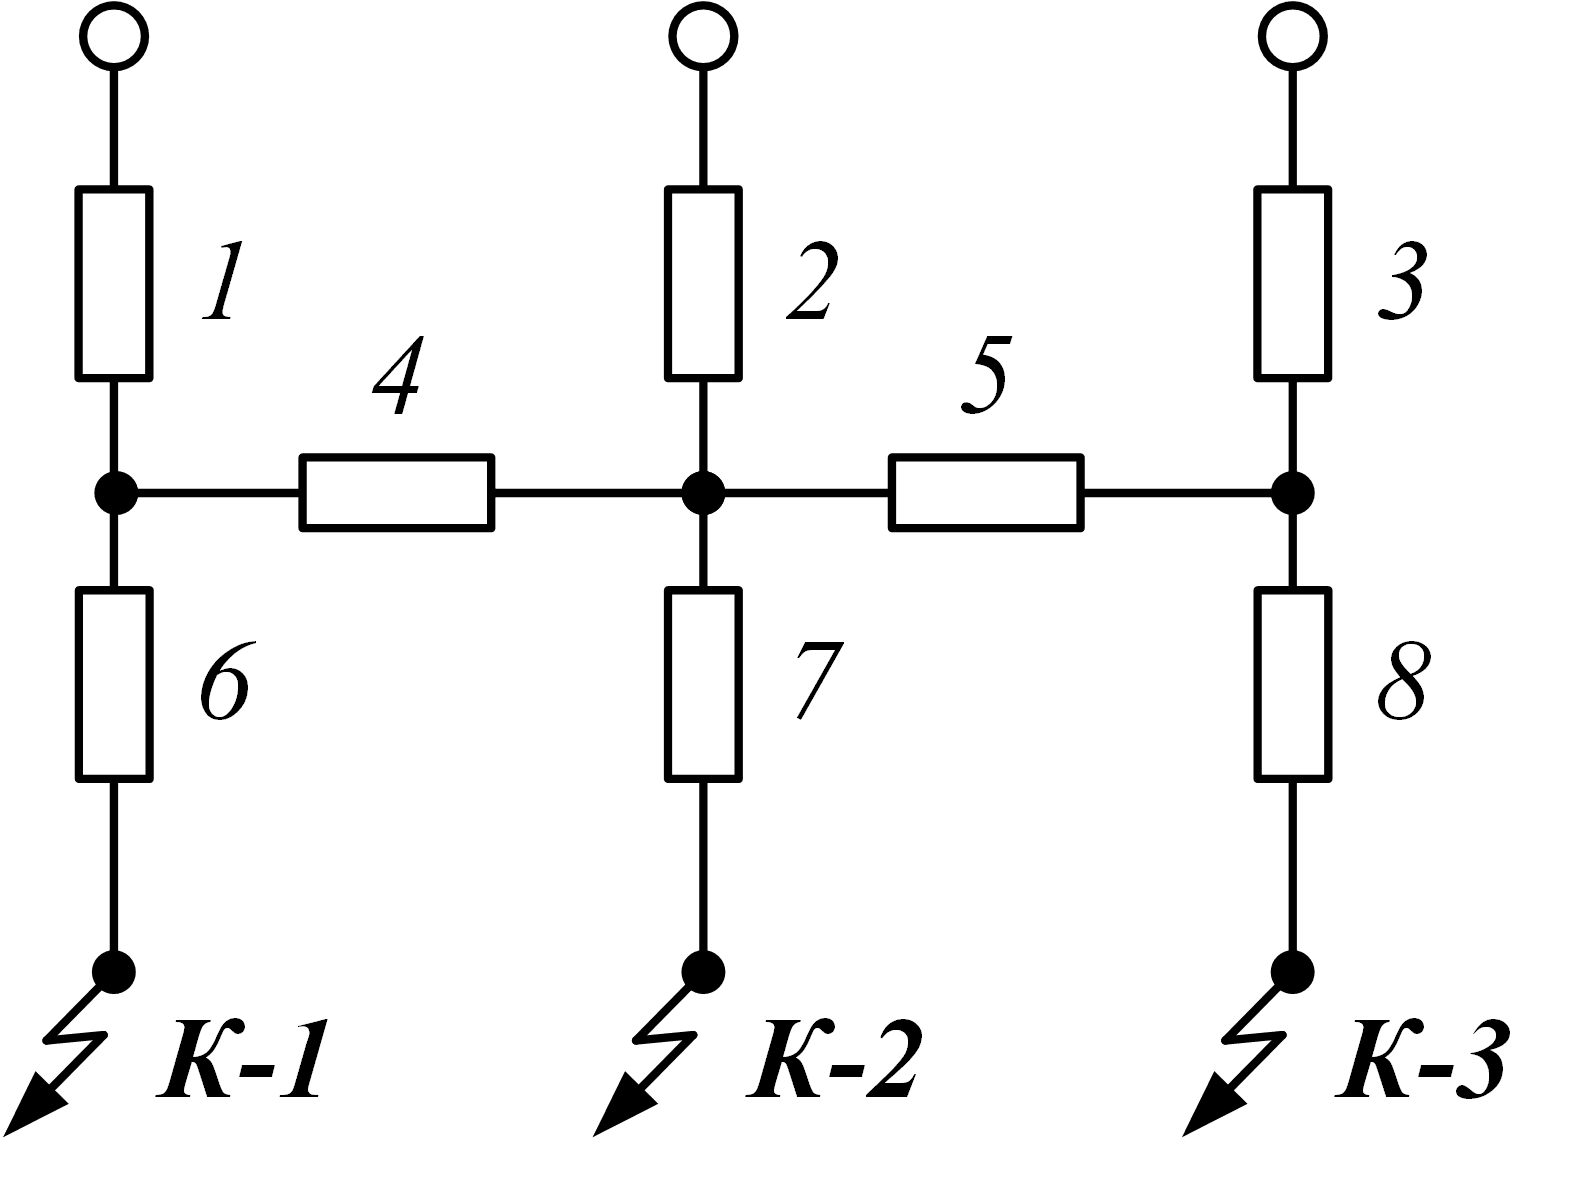
\includegraphics[width=1\linewidth]{pic/2-4_b}} \\ \textit{б)}
	\end{minipage}
	\vfill
	\begin{minipage}[h]{0.47\linewidth}
		\center{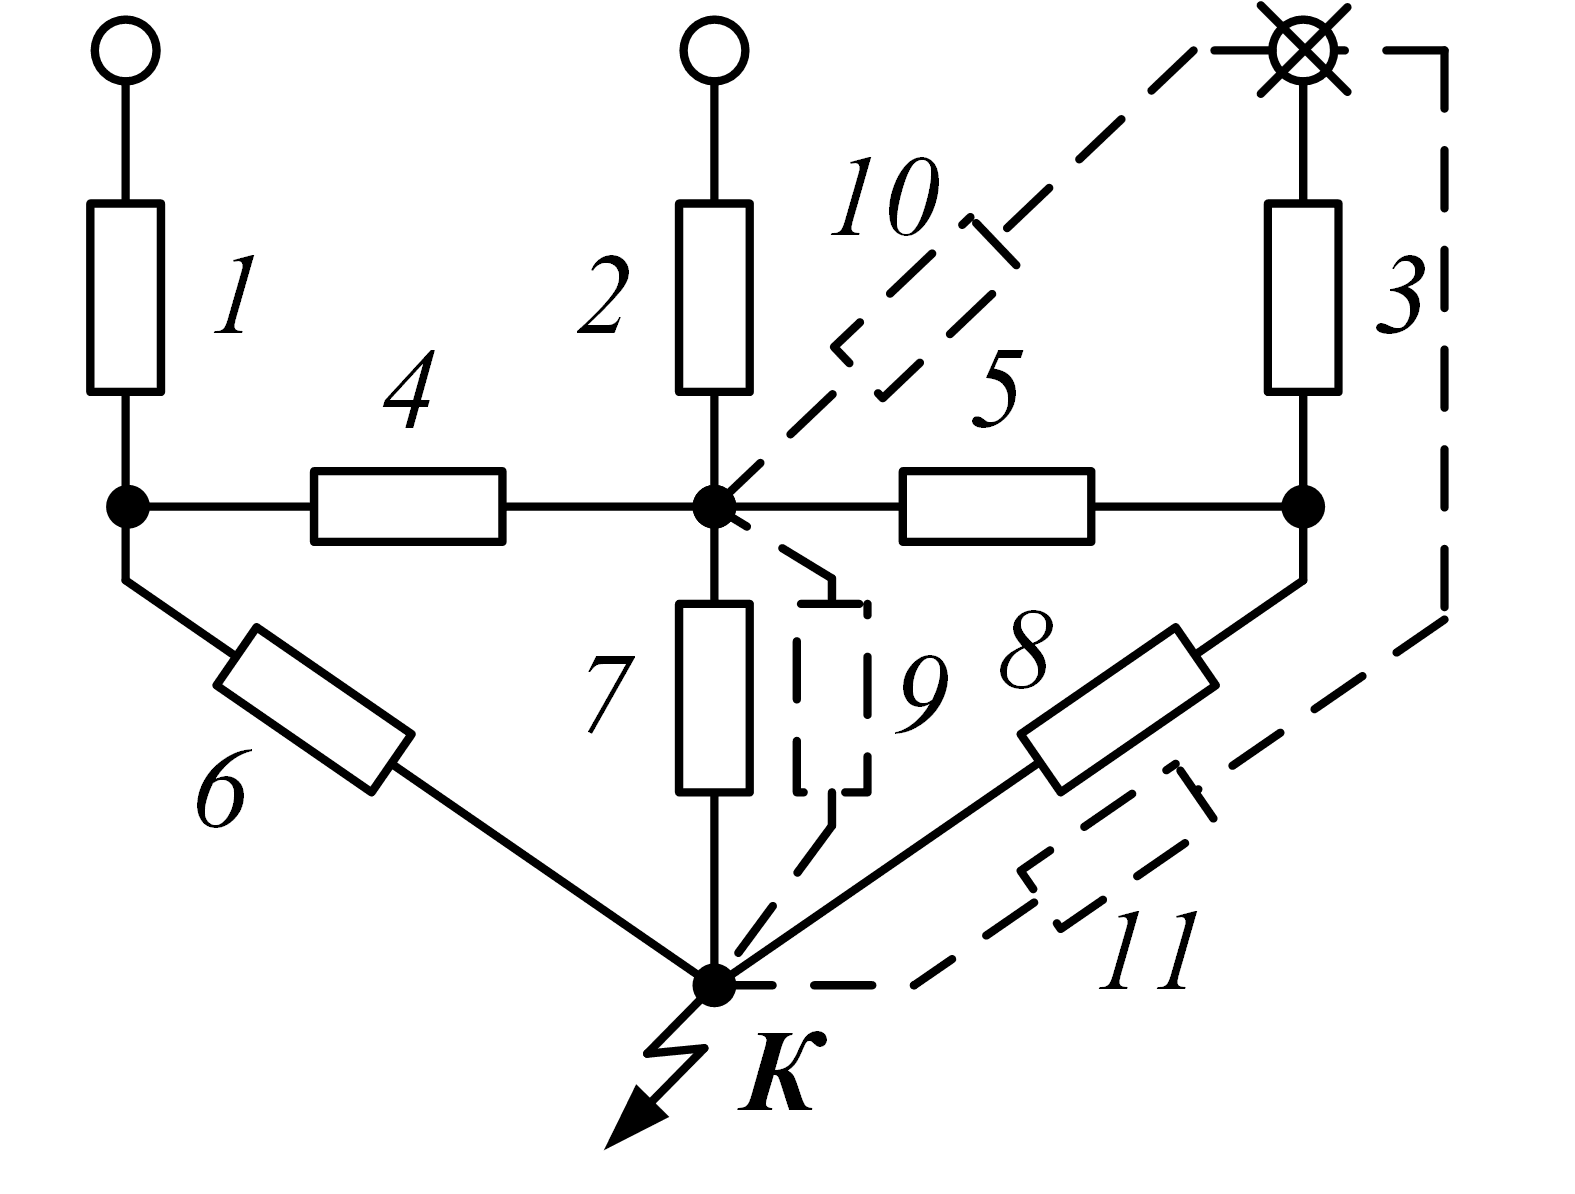
\includegraphics[width=1\linewidth]{pic/2-4_v}} \\ \textit{в)}
	\end{minipage}
	\hfill
	\begin{minipage}[h]{0.47\linewidth}
		\center{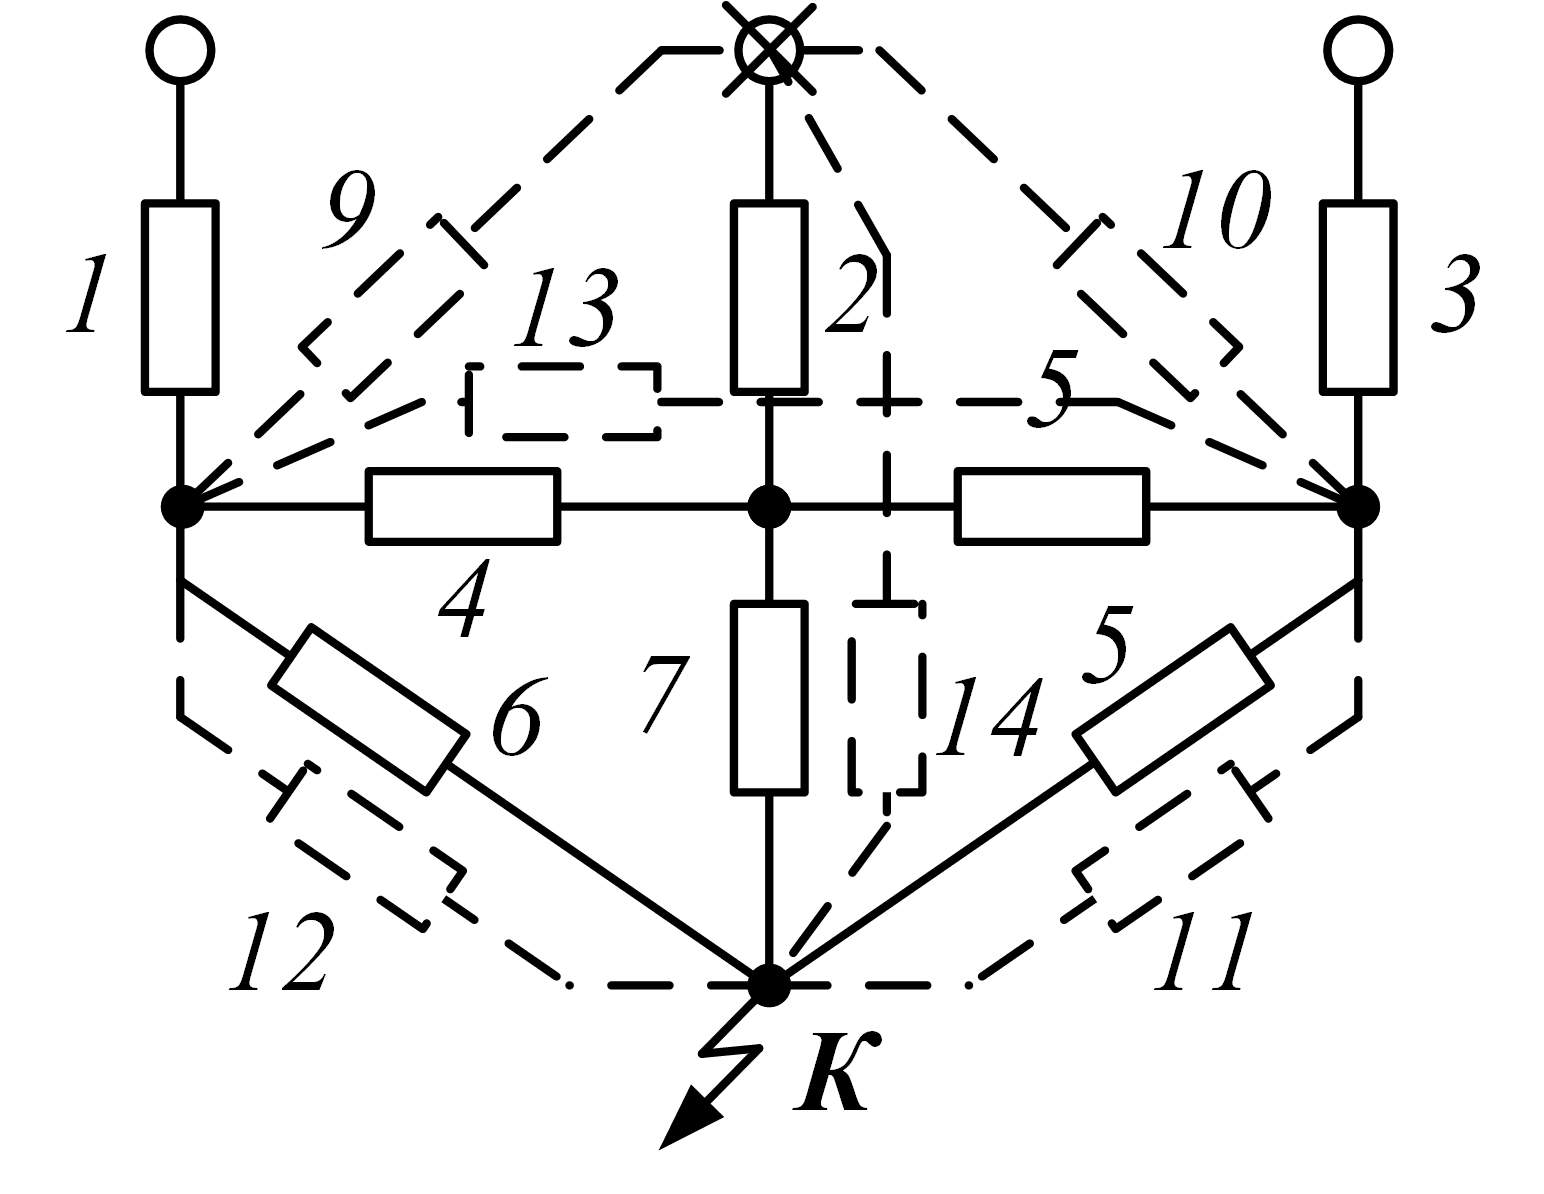
\includegraphics[width=1\linewidth]{pic/2-4_g}} \\ \textit{г)}
	\end{minipage}
	\caption{Пример преобразования схемы: \textit{а} --- исходная схема; \textit{б} --- после рассечения в узле короткого замыкания; \textit{в} и \textit{г} --- этапы преобразования схемы.}
	\label{ris:2-4 primer_preobrazovaniia_skhemy}
\end{figure}

В общем случае, когда элементы схемы рис.~\ref{ris:2-4 primer_preobrazovaniia_skhemy},\textit{а} различны, для ее упрощения можно одну из трехлучевых звезд с элементами \textit{1}, \textit{4}, \textit{6} или \textit{3}, \textit{5}, \textit{8} заменить эквивалентным треугольником (рис.~\ref{ris:2-4 primer_preobrazovaniia_skhemy},\textit{в}), затем разрезать его вершину, где приложена э.~д.~е., и образовавшиеся параллельные ветви (\textit{2} и \textit{10}, \textit{7} и \textit{9}) заменить эквивалентными. Еще одно преобразование оставшегося треугольника с последующим параллельным и последовательным сложением ветвей быстро приводит к цели. При желании можно четырехлучевую звезду \textit{2}, \textit{4}, \textit{5}, \textit{7} схемы рис.~\ref{ris:2-4 primer_preobrazovaniia_skhemy},\textit{а} преобразовать в четырехугольник с диагоналями (рис.~\ref{ris:2-4 primer_preobrazovaniia_skhemy},\textit{г}), а затем разрезать его вершину, где приложена э.~д.~е., и произвести замену параллельных ветвей. Однако в данном примере, как видно, такое преобразование не имеет преимуществ по сравнению с рассмотренным выше, хотя нужно заметить, что в более сложных схемах оно оказывается весьма эффективным, а иногда даже единственно возможным приемом упрощения схемы.

Все сказанное также относится к выполнению преобразований схем для расчета и других повреждений, как-то: обрыв проводов, одновременные повреждения в нескольких точках и т.~д.; причем если повреждения сопровождаются возникновением несимметрии трехфазной системы, то аналогичным преобразованиям подвергают схемы замещения всех последовательностей. Отметим, что при повреждении в двух точках элементарной схемой, к которой может быть приведена исходная схема, является либо треугольник, либо эквивалентная ему звезда (см. \colorbox{red}{§~16-4}).

С помощью расчетной модели суммарное или результирующее сопротивление схемы относительно любой ее точки легко находят непосредственным измерением. На ней также можно замерить сопротивления, по которым нетрудно определить параметры элементарной схемы при одновременных повреждениях в двух точках заданной системы.

\section{Применение принципа наложения}
\label{sec:2-6 primenenie_printcipa_nalozheniia}

В практических расчетах линейных электрических цепей часто представляется удобным использовать принцип наложения, согласно которому действительный режим можно получить как результат наложения ряда условных режимов, каждый из которых определяется в предположении, что в схеме приложена только одна (или группа) э.~д.~с, в то время как все остальные равны нулю; при этом все элементы схемы остаются включенными. Расчет каждого из таких условных режимов представляет более простую задач. Использование принципа наложения в такой обычной форме при достаточно большом числе различных э.~д.~с. в схеме становится громоздким и неудобным. Поэтому обычно на практике используют следующие формы принципа наложения.

\vspace{1pc}
\textit{а) Наложение собственно аварийного режима на предшествующий}

Условия трехфазного короткого замыкания не изменятся, если представить, что в точке короткого замыкания приложены две равные, но взаимно противоположные э.~д.~с. Их величина, вообще говоря, может быть произвольной; в частности, ее можно принять равной напряжению, которое было в этой точке до возникновения в ней короткого замыкания. Если генераторы введены в схему своими э.~д.~с, которые у них были до короткого замыкания, то режим после возникновения короткого замыкания удобно представить состоящим из двух режимов. Один из них целесообразно получить, учитывая все э.~д.~с. и дополнительно введенную в точку короткого замыкания э.~д.~с, равную $ + U_{\text{К0}} $. Одновременное действие этих э.~д.~с, очевидно, дает предшествующий режим в данной схеме. Второй режим получается от действия только одной э.~д.~с, приложенной в точке короткого замыкания и равной $ -U_{\text{К0}} $. Его называют собственно аварийным режимом, а получающиеся при нем токи и напряжения -- аварийными составляющими соответственно токов и напряжений.

Таким образом, суммируя предшествующие величины с собственно аварийными составляющими, получаем действительные величины при трехфазном коротком замыкании, т.~е.

\begin{equation}
	\label{eq:2-33 I_as_summ}
	\overset{\;.}{I} = \overset{\;.}{I}_0 + \overset{\;.}{I}_{AB};
\end{equation}

\begin{equation}
	\label{eq:2-34 U_as_summ}
	\overset{\;.}{U} = \overset{\;.}{U}_0 + \overset{\;.}{U}_{AB}.
\end{equation}

Здесь $ U < \overset{\;.}{U}_0 $, поскольку $ U_{AB} < 0 $. Что касается токов, то в генераторах $ I_{AB} $ имеют одно направление с $ I_0 $, а во всех прочих ветвях эти токи могут иметь как одинаковые, так и разные направления.

Использование такой формы наложения особенно эффективно в случаях, когда предшествующий режим уже известен; при этом задача сводится к сравнительно более простому расчету только собственно аварийного режима. На практике часто допускают наложение собственно аварийного режима, полученного для чисто индуктивной схемы, на предшествующий режим, который соответствует схеме с полными сопротивлениями ее элементов. Разумеется, такое наложение принципиально неточно, однако в большинстве случаев им можно пользоваться, поскольку получающиеся ошибки незначительны\footnote{Это объясняется тем, что аварийные составляющие токов обычно много больше токов предшествующего режима.}.

Нужно подчеркнуть, что если собственно аварийные составляющие токов отдельных ветвей в общем случае являются фиктивными токами, то сумма этих составляющих генераторных и нагрузочных ветвей образует действительный ток в месте короткого замыкания, так как в нем до возникновения короткого замыкания ток отсутствовал. Поэтому когда задача ограничена определением тока только в месте короткого замыкания, то его можно найти, исходя из предшествующего напряжения в аварийной точке, причем если последнее неизвестно, то, вообще говоря, им можно задаться, имея в виду, что в нормальном режиме отклонения напряжения сравнительно малы.

Рассматриваемую форму принципа наложения также можно использовать в расчетах простых и сложных несимметричных режимов (см.~\colorbox{red}{§ 13-5}).

%TODO: Нарисовать картинку 2-5
\begin{figure}[h]
	\begin{minipage}[h]{0.5\linewidth}
		\center{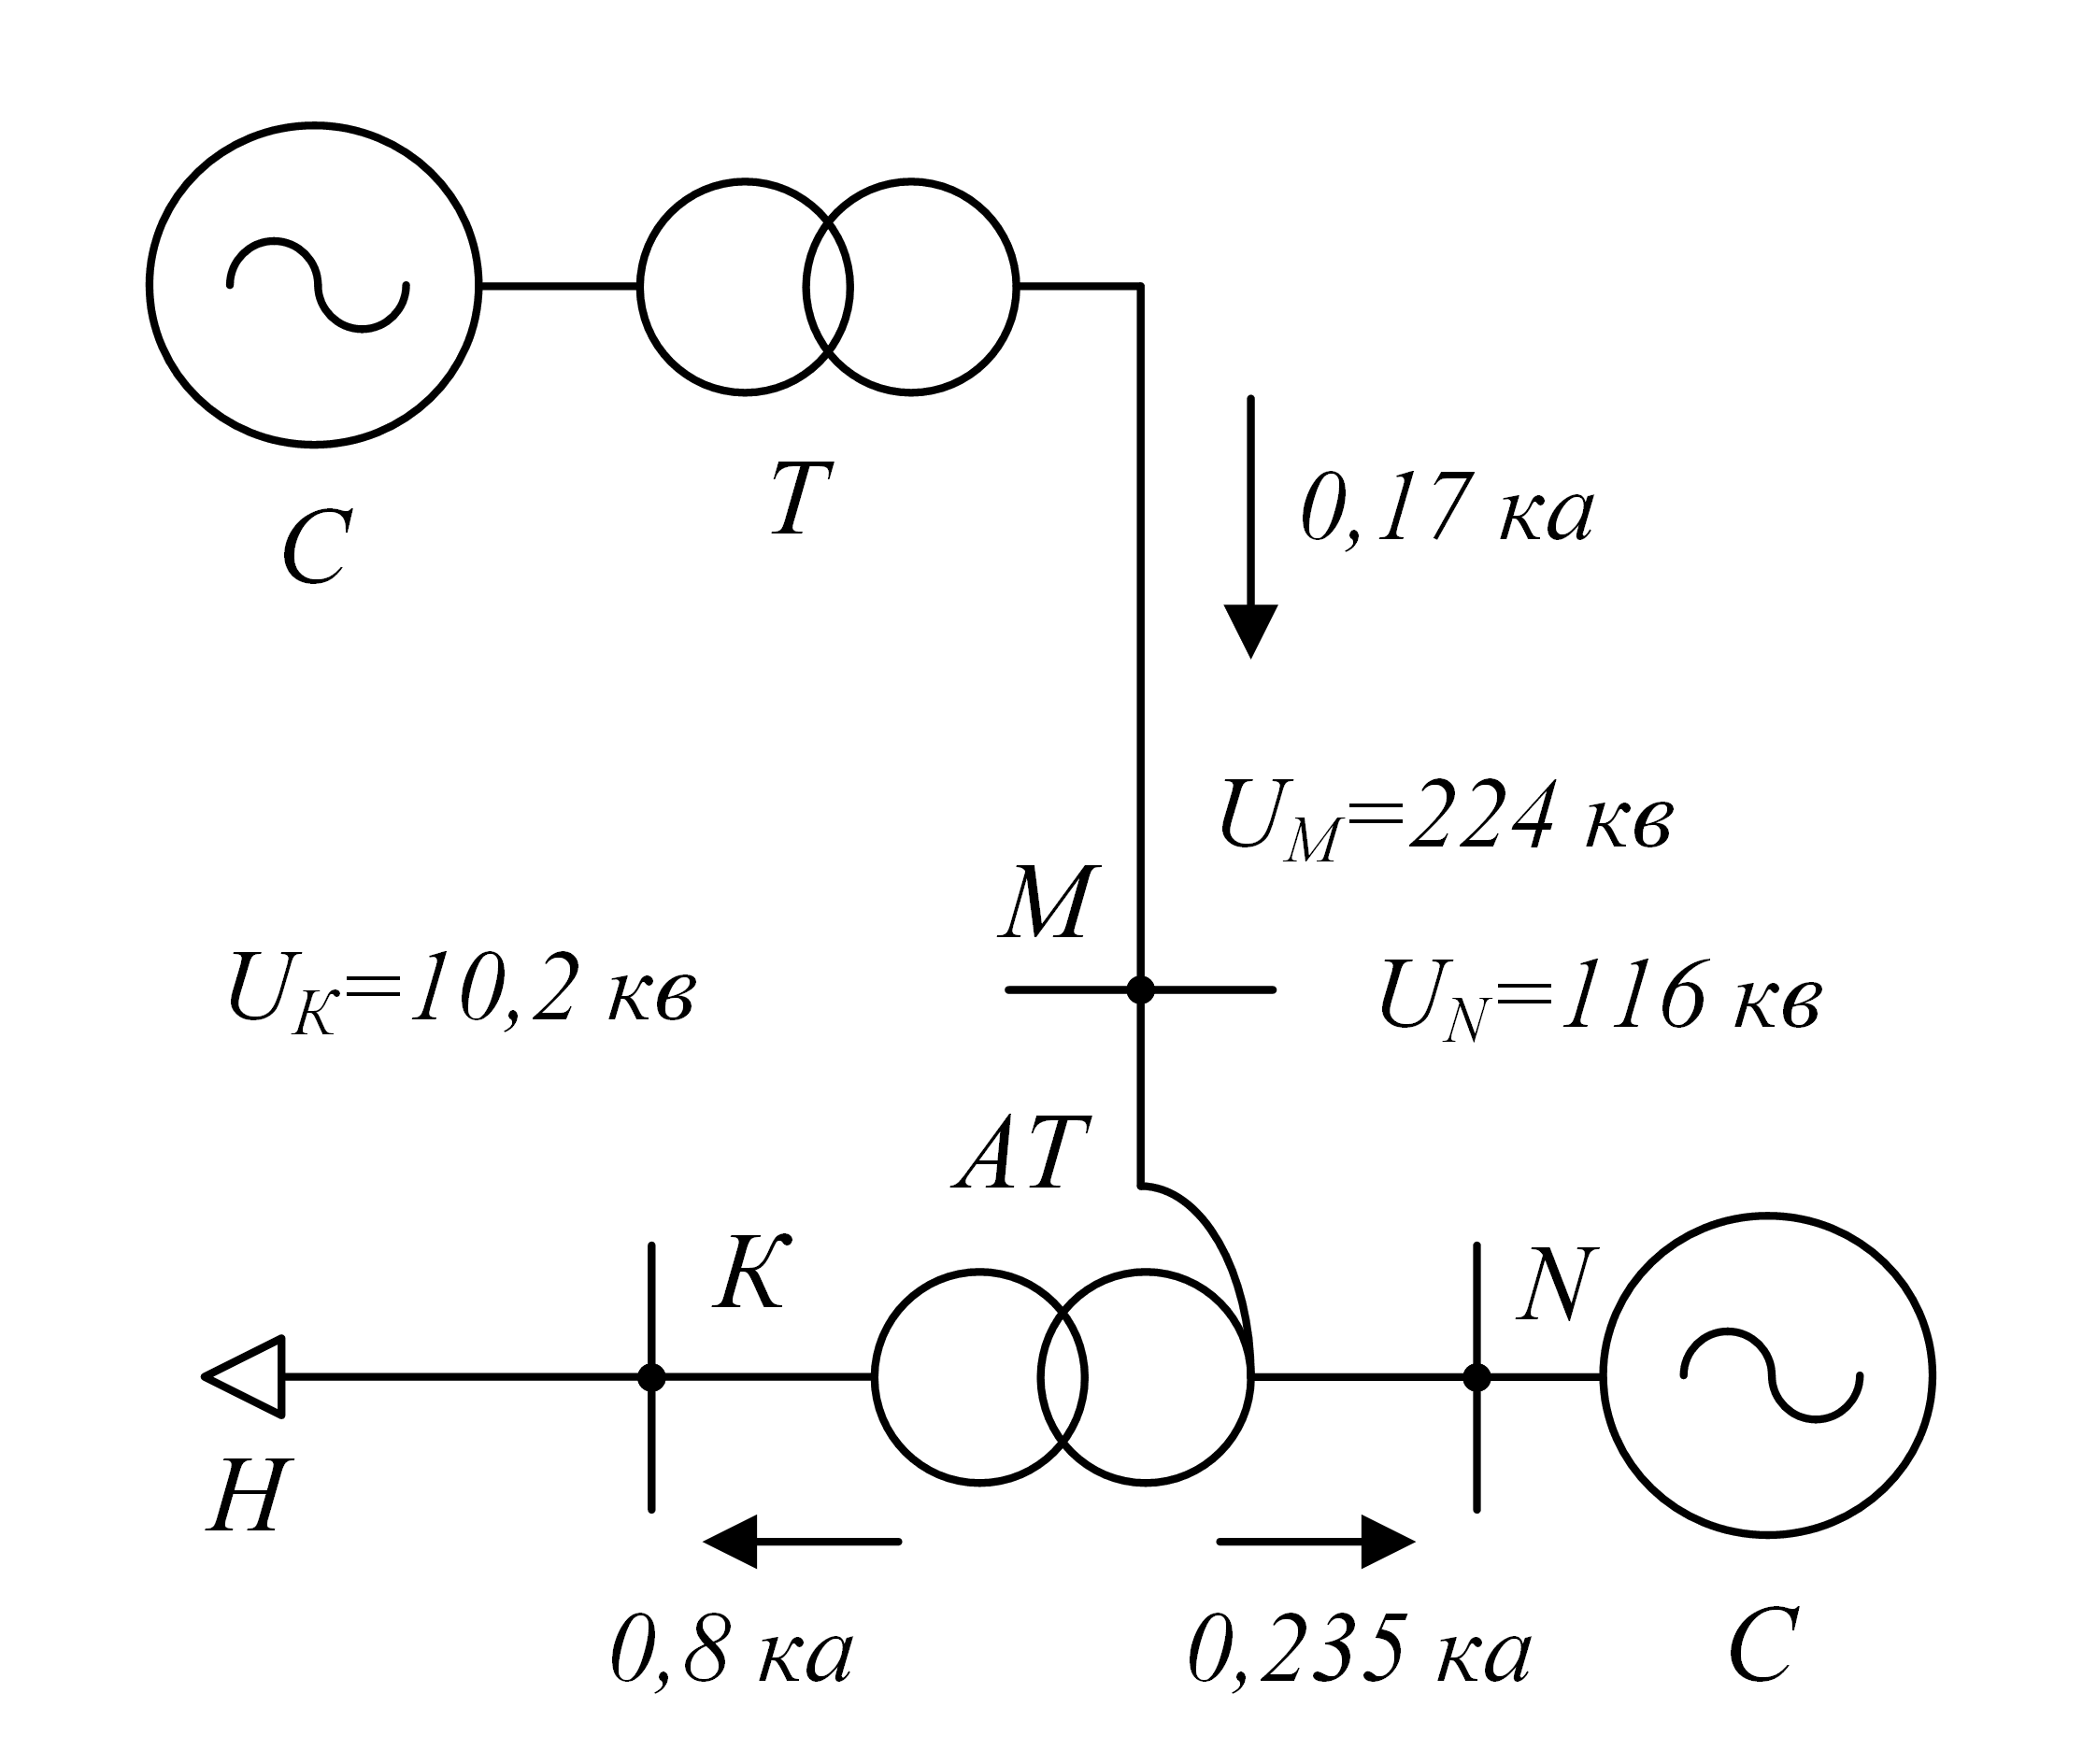
\includegraphics[width=1\linewidth]{pic/2-5_a} \\ \textit{а})}
	\end{minipage}
	\hfill
	\begin{minipage}[h]{0.5\linewidth}
		\center{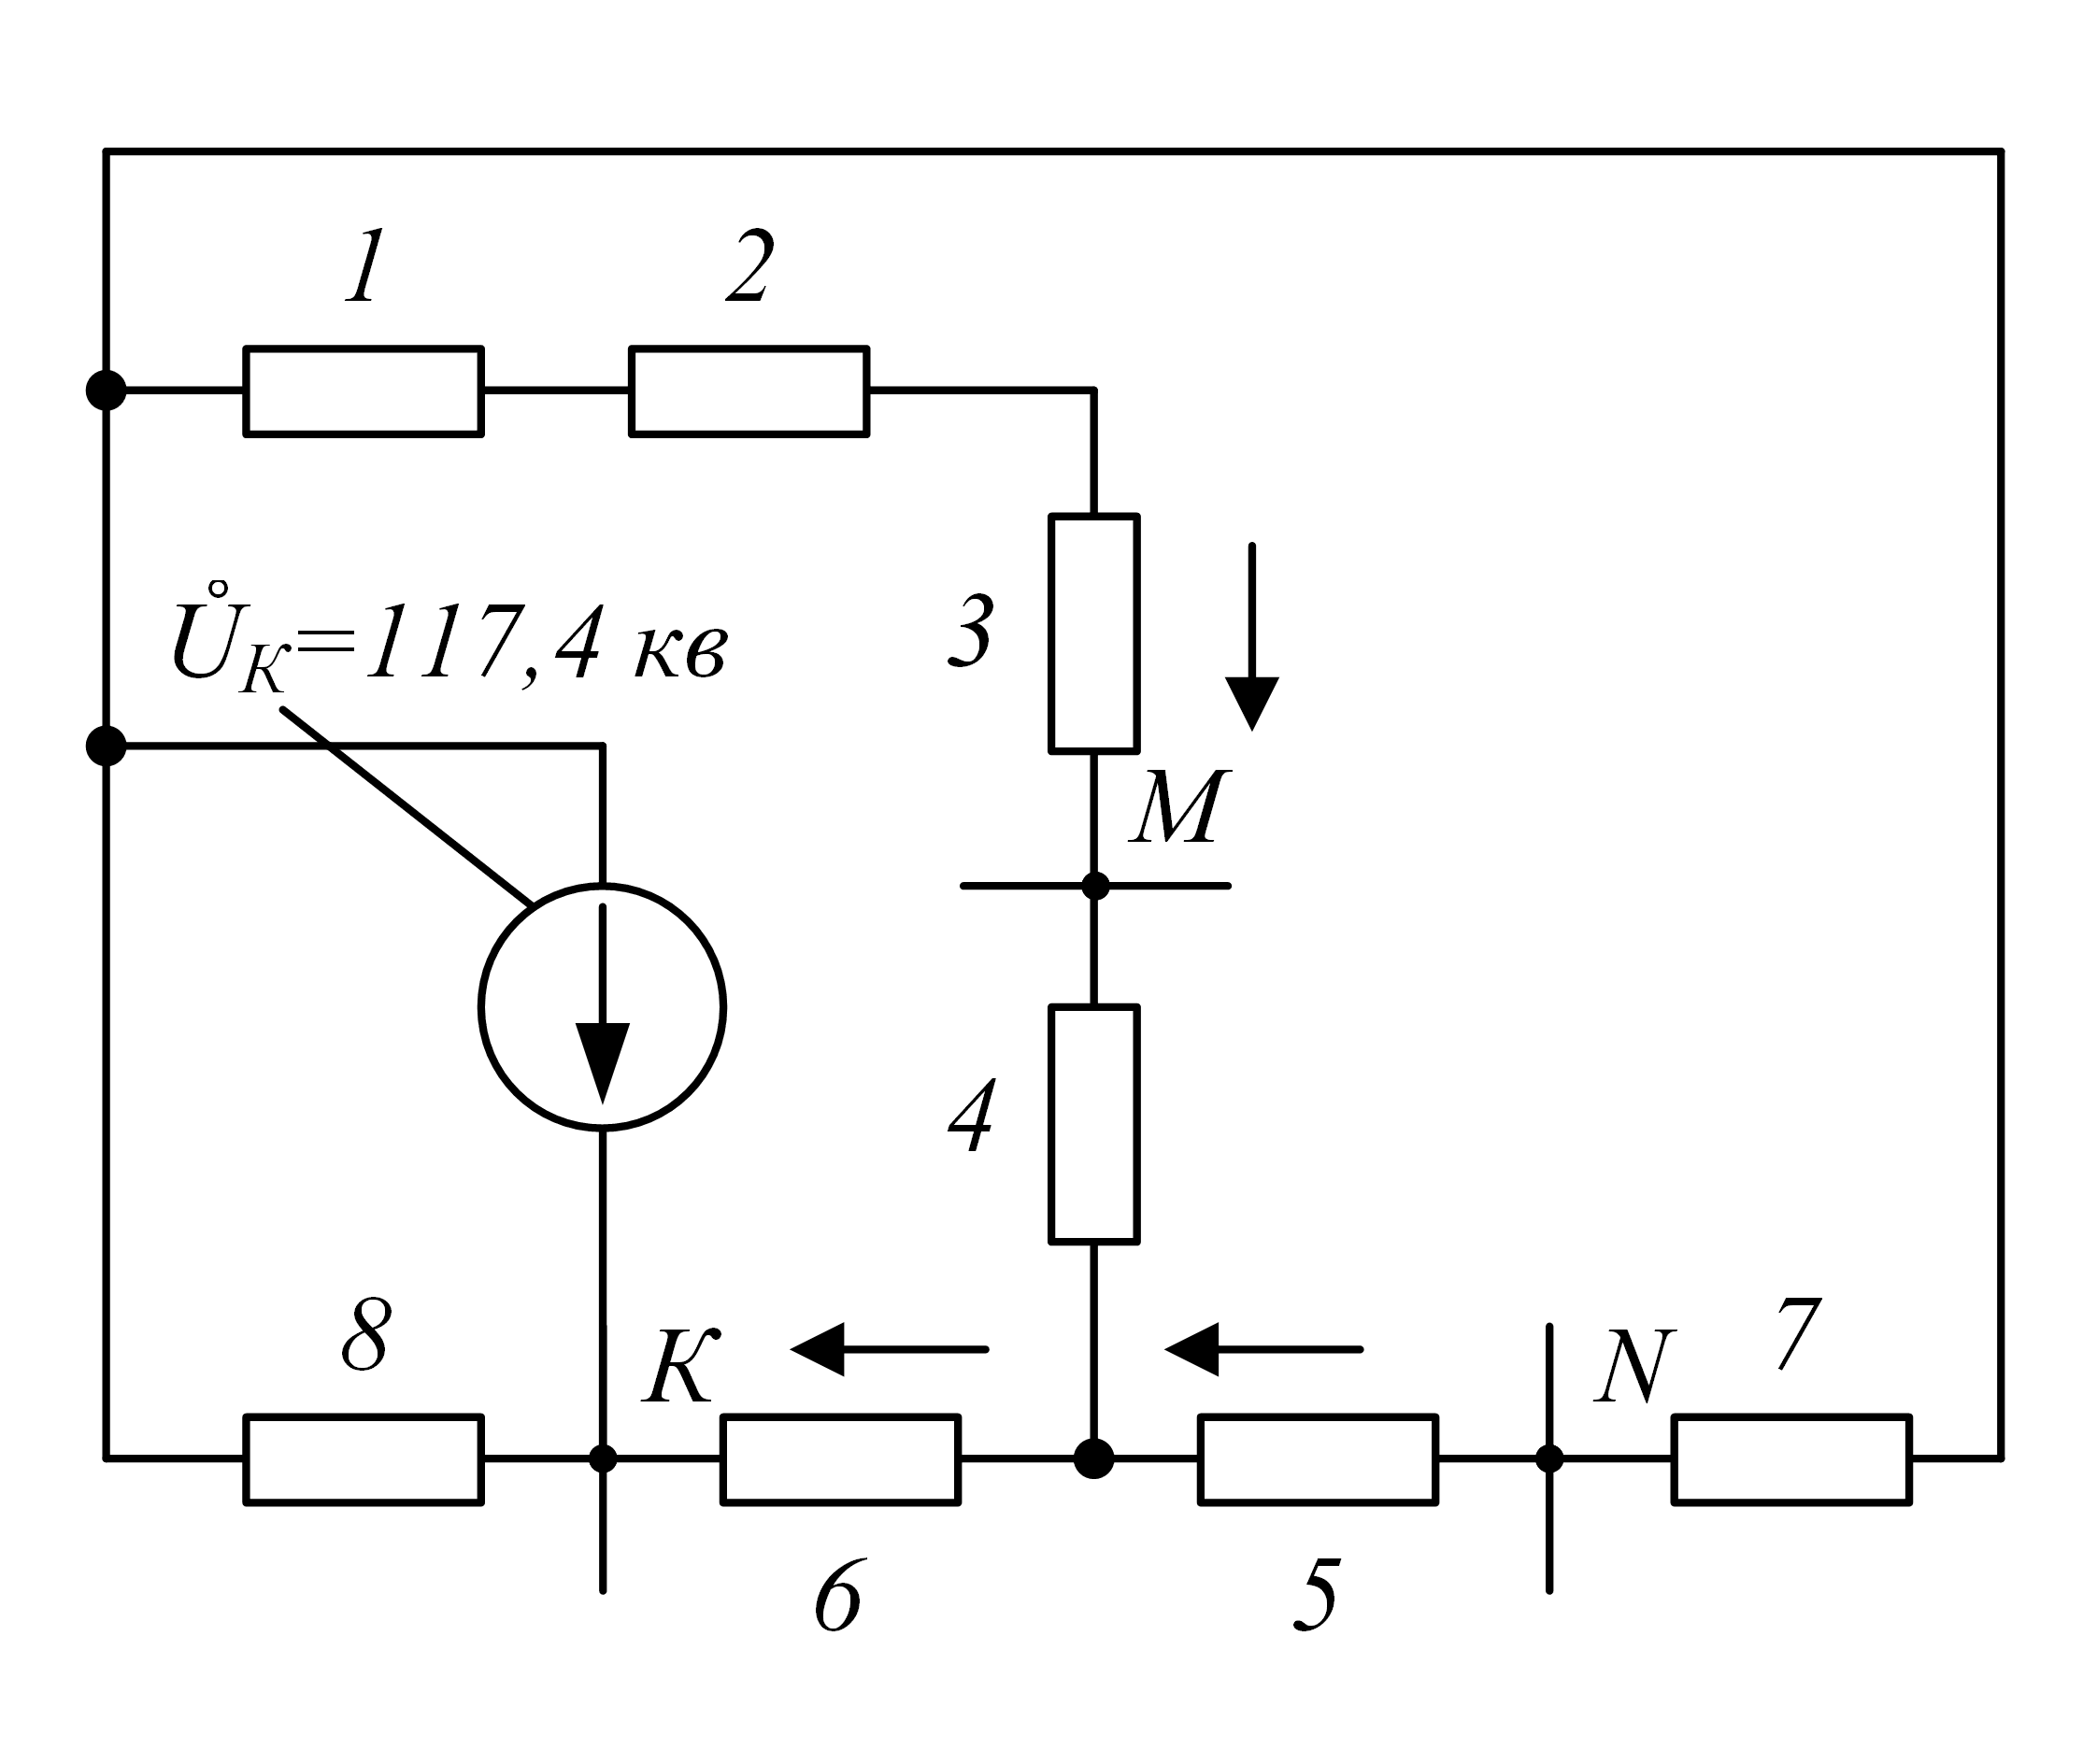
\includegraphics[width=1\linewidth]{pic/2-5_b} \\ \textit{б})}
	\end{minipage}
	\caption{К примеру \ref*{chap:2 obshchie ukazaniia k vypolneniiu raschetov}-\arabic{example}}
	\label{ris:2-5 k_primeru_2-3}
\end{figure}

\addtocounter{example}{1}

\begin{small} % пример 2-3
	
	\label{exmpl:2-3}
	\vspace{1pc}
	\textit{Пример \ref*{chap:2 obshchie ukazaniia k vypolneniiu raschetov}-\arabic{example}}. Для схемы рис.~\ref{ris:2-5 k_primeru_2-3},\textit{а} известны величины токов (\textit{ка}) и напряжений (\textit{кв}) предшествующего режима; они указаны на самой схеме.
	
	При трехфазном коротком замыкании в точке \textit{К} определить для начального момента периодическую слагающую тока в месте короткого замыкания и цепях автотрансформатора \textit{AT}; кроме того, для тех же условий найти линейные напряжения в точках \textit{М} и \textit{N}. Для упрощения считать, что заданные токи чисто индуктивные.
	
	Генератор \textit{Г} 194~\textit{Мва}; 18~\textit{кв}; $ x''_d = 0,235 $ {\renewcommand{\thefootnote}{*}\footnote{Эта реактивность характеризует генератор в начальный момент переходного процесса (\colorbox{red}{см. § 6-2 и 6-3}).}}\addtocounter{footnote}{-1}
	
	Трансформатор \textit{Т} 200~\textit{Мва}; 242/18~\textit{кв}; $ u_\text{К} = 12 \% $.
	
	Автотрансформатор \textit{АТ} 125~\textit{Мва}; 220/121/11~\textit{кв}; $ u_\text{ВС} = 10,5 \% $; $ u_\text{ВН} = 36,3 \% $, $ u_\text{СН} = 23 \% $.
	
	Линия 135~\textit{км}; $ x = 0,4 $~\textit{ом/км}.
	
	Система \textit{С} --- эквивалентная реактивность $ x = 10 $~\textit{ом}.
	
	Проведем решение в именованных единицах, выбрав в качестве основной ступень линии передачи.
	
	Схема замещения для собственно аварийного режима представлена на рис.~\ref{ris:2-5 k_primeru_2-3},\textit{б}. Введенное в нее напряжение в точке короткого замыкания определено как
	
	\begin{equation*}
		\overset{\;\circ}{U} = - \frac{10,2}{\sqrt{3}} \cdot -117,4 \text{~\textit{кв}}.
	\end{equation*}
	
	Реактивности всех элементов схемы рис.~\ref{ris:2-5 k_primeru_2-3},\textit{б} составляют $ x_1 = 71 $~\textit{ом}; $ x_2 = 35,2 $~\textit{ом}; $ x_3 = 54 $~\textit{ом}; $ x_4 = 46 $~\textit{ом}; $ x_5 = -5,4 $~\textit{ом}; $ x_6 = 94,5 $~\textit{ом}; $ x_7 = 33,2 $~\textit{ом}; $ x_8 = \frac{10,2}{2 \cdot 0,8} \cdot \big(\frac{220}{11}\big)^2 = 2940 $~\textit{ом}.
	
	Определим результирующую реактивность схемы относительно точки \textit{К}: $ x_9 = 71 + 35,2 + 54 + 46 = 206,2 $~\textit{ом}; \hspace{1pc} $ x_10 = 33,2 - 5,4 = 27,8 $~\textit{ом}; \hspace{1pc} $ x_11 = 206,2 // 27,8 = 24,5 $~\textit{ом}; \hspace{1pc} $ x_12 = 24,5 + 94,5 = 119 $~\textit{ом}; и $ x_{\sum} = 119 // 2940 = 114 $~\textit{ом}{\renewcommand{\thefootnote}{**}\footnote{Знак // --- условная запись параллельного сложения ветвей.}}\addtocounter{footnote}{-1}.
	
	Ток в месте короткого замыкания $ \overset{\;\circ}{I}_K = \frac{0 - (-117,4)}{114} = 1,03 $~\textit{ка} и его истинное значение $ I_K = 1,03 \cdot \frac{220}{11} = 20,6 $~\textit{ка}.
	
	Распределение собственно аварийной составляющей тока будет:
	
	\begin{equation*}
		I_{\text{ав8}} = \frac{-117,4}{2940} = -0,04 \textit{~ка};
		\hspace{1pc}
		I_{\text{ав6}} = 1,03 - 0,04 = 0,99 \textit{~ка};		
	\end{equation*}
	
	\begin{equation*}
		I_{\text{ав5}} = 0,99 \cdot \frac{24,5}{27,8} = 0,87 \textit{~ка};
		\hspace{1pc}
		I_{\text{ав4}} = 0,99 - 0,87 = 0,12 \textit{~ка}.		
	\end{equation*}
	
	Искомые токи будут:
	
	на стороне высшего напряжения $ I = 0,12 + 0,17 = 0,29 \textit{~ка} $;
	
	на стороне среднего напряжения $ I = 0,87 \frac{220}{121} - 0,235 = 1,345 \textit{~ка} $; 
	
	на стороне низшего напряжения $ I = 0,99 \frac{220}{11} + 0,8 = 20,6 \textit{~ка} $, т.~е. как и следовало ожидать, та же величина, что и в месте короткого замыкания. 	
	
	Аварийные составляющие напряжений:
	
	в точке \textit{М}
	
	\begin{equation*}
		U_{\text{ав\textit{М}}} = -0,12 (71 + 35,2 + 54) = -19,2 \textit{~кв};
	\end{equation*}	

	в точке \textit{N}
	
	\begin{equation*}
		U_{\text{ав\textit{N}}} = -0,87 \cdot 33,2 = -28,9 \textit{~кв}.
	\end{equation*}	

	Искомые величины линейных напряжений будут:
	
	в точке \textit{М}
	
	\begin{equation*}
		U_M = 224 - \sqrt{3} \cdot 19,2 = 191 \textit{~кв} \text{ (снижение примерно на 15\%)};
	\end{equation*}	

	в точке \textit{N}
	
	\begin{equation*}
		U_N = 116 - \sqrt{3} \cdot 28,9 \cdot \frac{121}{220} = 88,5 \textit{~кв} \text{ (снижение примерно на 24\%)};
	\end{equation*}		

\end{small}


\vspace{1pc}
\textit{б) Применение собственных и взаимных сопротивлений и проводимостей }

В схеме с произвольным числом источников с э.~д.~с. $ \overset{~.}{E}_1, \overset{~.}{E}_2, \ldots, \overset{~.}{E}_n $ для тока, например, источника \textit{1}, считая положительным напряжение тока от источника к внешней сети, по принципу наложения можно записать:

%TODO: Здесь бы нужно использовать многострочные формулы
\begin{equation*}
	\overset{~.}{I}_1 = \overset{~.}{I}_{11} - \overset{~.}{I}_{12} - \overset{~.}{I}_{13} - \ldots - \overset{~.}{I}_{1n} = \frac{\overset{~.}{E}_{1}}{Z_{11}} - \frac{\overset{~.}{E}_{2}}{Z_{12}} - \frac{\overset{~.}{E}_{3}}{Z_{13}} -
\end{equation*}	
\begin{equation*}
	- \ldots - \frac{\overset{~.}{E}_{n}}{Z_{1n}} = Y_{11}\overset{~.}{E}_1 - Y_{12}\overset{~.}{E}_2 - Y_{13}\overset{~.}{E}_3 - 
\end{equation*}	
\begin{equation}
	- \ldots - Y_{1n}\overset{~.}{E}_n, 
	\label{eq:2-35 summa_tokov}
\end{equation}

где каждый из токов обусловлен действием лишь одной э.~д.~с. при равенстве нулю всех прочих, т.~е.

$ \overset{~.}{I}_{11} = \frac{\overset{~.}{E}_1}{Z_{11}} = Y_{11}\overset{~.}{E}_1 $ --- собственный ток источника \textit{1}, созданный только его э.~д.~с. $ \overset{~.}{E}_1 $;

$ \overset{~.}{I}_{12} = \frac{\overset{~.}{E}_2}{Z_{12}} = Y_{12}\overset{~.}{E}_2 $ --- взаимный ток источника \textit{1}, вызванный только э.~д.~с. $ \overset{~.}{E}_2 $ и т.~д.

Здесь $ Z_{11}, Z_{12}, \ldots, Z_{1n} $ и $ Y_{11}, Z_{12}, \ldots, Z_{1n} $ --- соответственно собственные и взаимные сопротивления и проводимости источника \textit{1} в рассматриваемой схеме.

Аналогично для тока в месте короткого замыкания имеем:

\begin{equation*}
	\overset{~.}{I}_{К} = \frac{\overset{~.}{E}_1}{Z_{1\text{К}}} + \frac{\overset{~.}{E}_2}{Z_{2\text{К}}} + \ldots + \frac{\overset{~.}{E}_n}{Z_{n\text{К}}} =
\end{equation*}	
\begin{equation}
	= Y_{1\text{К}}\overset{~.}{E}_1 + Y_{2\text{К}}\overset{~.}{E}_2 + \ldots + Y_{n\text{К}}\overset{~.}{E}_n,
	\label{eq:2-36 summa_tokov}
\end{equation}
  
где $ Z_{1\text{К}}, Z_{2\text{К}}, \ldots, Z_{n\text{К}} $ и $ Y_{1\text{К}}, Z_{2\text{К}}, \ldots, Z_{n\text{К}} $ --- взаимные сопротивления и проводимости между каждым источником и точкой короткого замыкания.

Выражения (\ref{eq:2-35 summa_tokov}) и (\ref{eq:2-36 summa_tokov}) особенно удобны, когда требуется выявить индивидуальные свойства отдельных источников или учесть влияние изменения величины и фазы отдельных э.~д.~с. на искомые значения токов.

Собственные и взаимные сопротивления или проводимости находят с помощью так называемого способа токораспределения или путем постепенного преобразования заданной схемы. Оба эти приема иногда целесообразно использовать совместно, т.~е. вначале произвести ряд преобразований схемы, а затем применить способ токораспределения. Сущность и применение этих приемов ниже иллюстрировано на конкретном примере.

В расчетах коротких замыканий часто приходится определять только взаимные сопротивления между точкой короткого замыкания и отдельными источниками (или группами их). Для этого удобно использовать следующий прием. Приняв ток в месте короткого замыкания за единицу и считая все приведенные э.~д.~с. одинаковыми, нужно произвести распределение этого тока (равного единице) в заданной схеме. Полученные доли этой единицы для отдельных источников: $ C_1, C_2, \ldots, C_n $, называемые \so{коэффициентами распределения}, при отсутствии нагрузок в схеме характеризуют долю участия каждого источника\footnote{Как отмечалось выше, при равенстве их приведенных э.~д.~с.} в питании короткого замыкания. Далее, если результирующее сопротивление схемы относительно места короткого замыкания $ Z_{\sum} $, то, очевидно, можно записать равенства:

\begin{equation*}
	C_1 Z_{1\text{К}} = C_2 Z_{2\text{К}} = \ldots = C_n Z_{n\text{К}} = 1 \cdot Z_{\sum},
\end{equation*}	

откуда искомое взаимное сопротивление между точкой короткого замыкания и соответствующим источником будет:

%TODO: Какая-то звездочка над формулой, проверить
\begin{equation}
	Z_{n\text{К}} = \frac{Z_{\sum}}{C_n}.
	\label{eq:2-37 Z_nK}
\end{equation}	

Нетрудно убедиться, что для нахождения собственного сопротивления каждого источника достаточно сложить параллельно все его взаимные сопротивления.

Расчетная модель позволяет значительно скорее и проще найти собственные и взаимные сопротивления и коэффициенты распределения. Попутно отметим, что последние особенно удобны для определения распределения токов обратной и нулевой последовательностей (\colorbox{red}{см.~§13-5}).

\addtocounter{example}{1}

\begin{small} % пример 2-4
	
	\label{exmpl:2-4}
	\vspace{1pc}
	\textit{Пример \ref*{chap:2 obshchie ukazaniia k vypolneniiu raschetov}-\arabic{example}}.
	Для схемы рис.~\ref{ris:2-6 k_primeru_2-4},\textit{а}, где у каждого элемента указана его реактивность, требуется определить:
	

	\begin{enumerate}
		\renewcommand{\labelenumi}{\asbuk{enumi})}  % делаем список, нумерованный буквами кириллического алфавита
		\item величины собственной реактивности относительно узла \textit{1} и взаимных реактивностей между этим узлом и узлами \textit{2}, \textit{3}, \textit{4} и \textit{5}, используя способ токораспределения;
		\item те же величины используя способ преобразования схемы;
		\item коэффициенты распределения и взаимные реактивности между точками \textit{1}, \textit{2}, \textit{4}, \textit{5} (где имеются источники) и точкой \textit{3} (где предполагается потенциал, равный нулю).		
	\end{enumerate}

	Проведем решение в указанной последовательности.

	\begin{enumerate}
		\renewcommand{\labelenumi}{\asbuk{enumi})}
		\item Считаем, что только в точке 1 расположена некоторая э.~д.~с. Через остальные конечные точки осуществляем замкнутый контур (рис.~\ref{ris:2-6 k_primeru_2-4},\textit{б}). Пусть $ I_3 = 1 $; тогда напряжение $ U_b = 1,5 $ и токи $ I_2 = \frac{1,5}{1,74} = 0,86 $ и $ I_4 = 1,5 / 0,79 = 1,9 $; на участке \textit{ab} $ I_{ab} = 1 + 1,9 + 0,86 = 3,76 $. Напряжение $ U_a = 1,5 + 0,5 \cdot 3,76 = 3,38 $; токи $ I_5 = 3,38 / 4,56 = 0,74 $ и $ I_1 = 3,76 + 0,74 = 4,5 $; э.~д.~с. $ E_1 = 3,38 + 4,5 \cdot 0,4 = 5,2 $.
		
		\begin{figure}[]
			\begin{minipage}[]{0.4\linewidth}
				\center{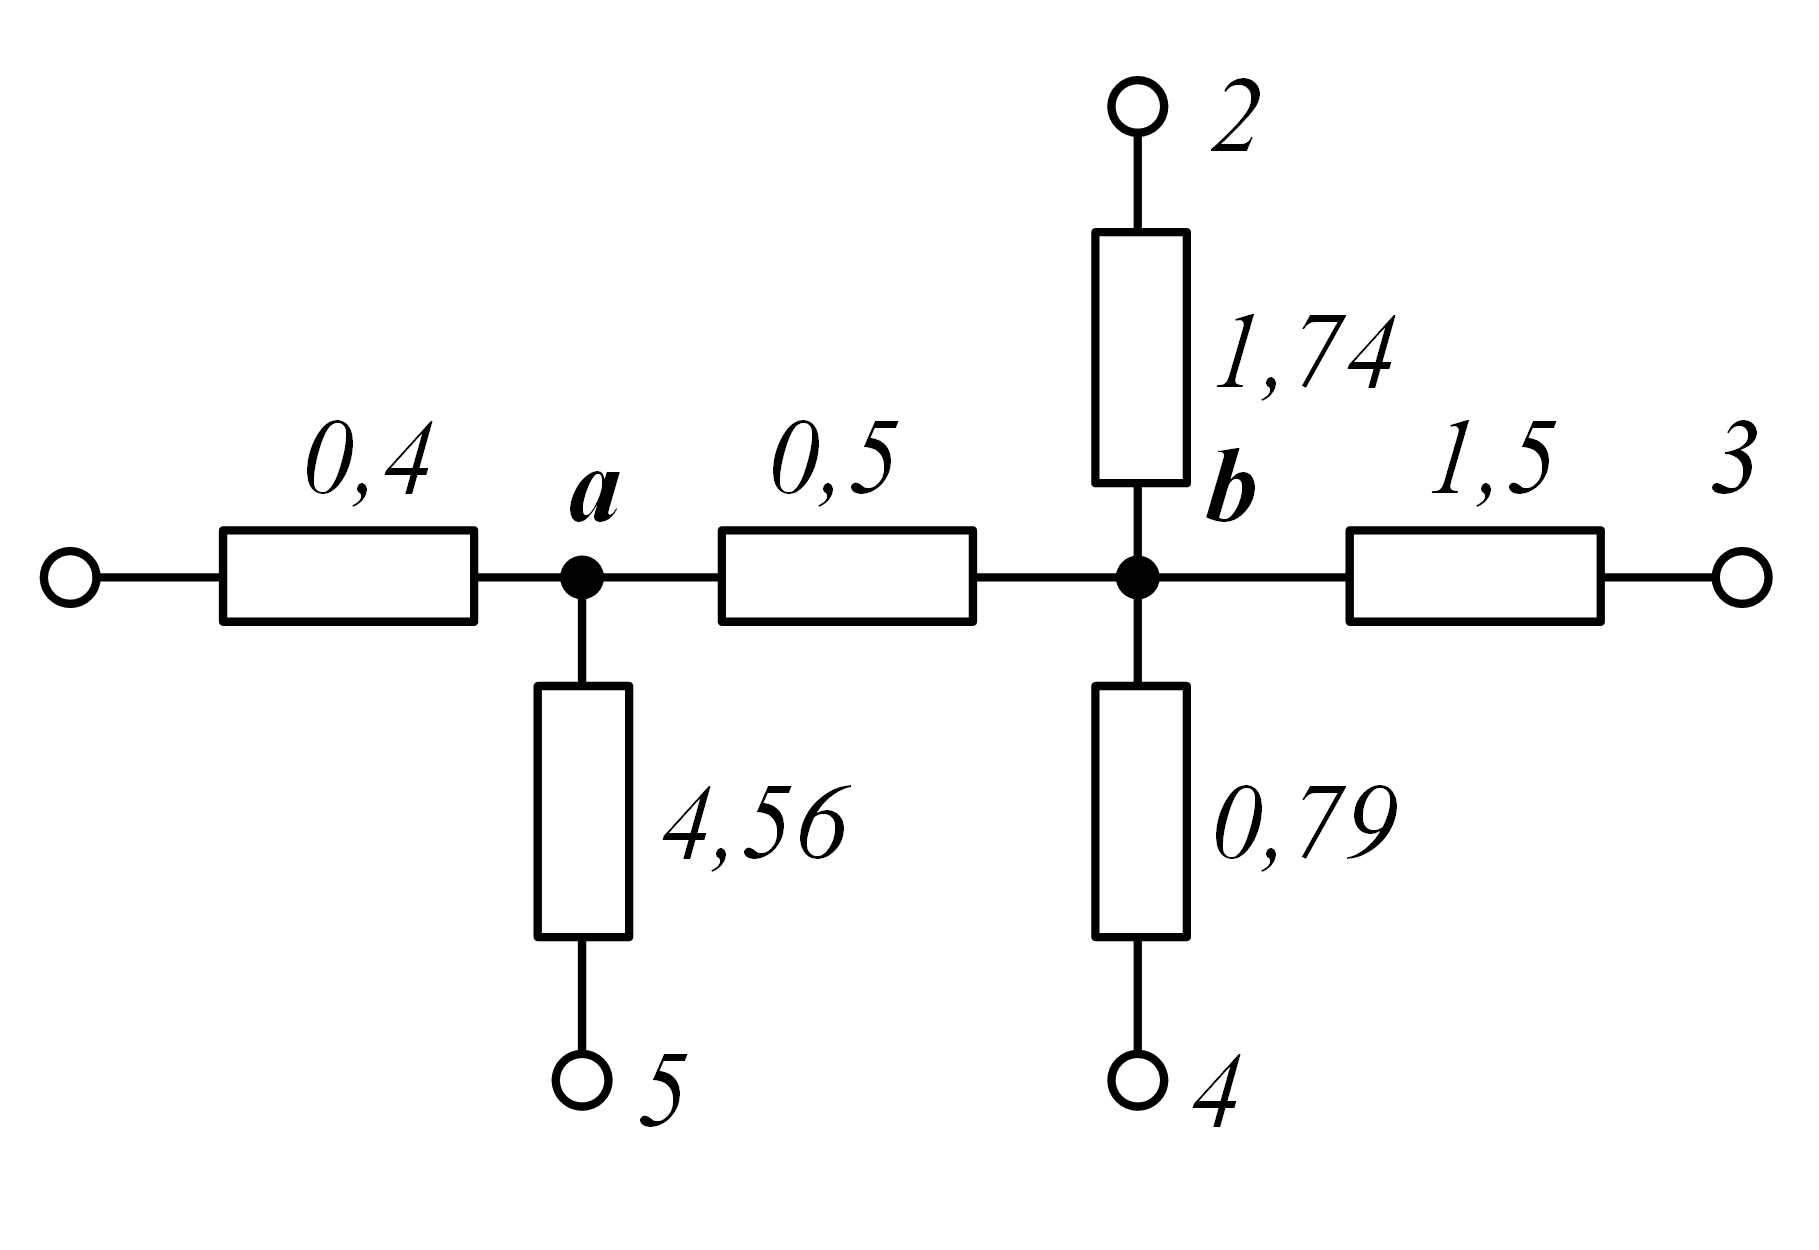
\includegraphics[width=1\linewidth]{pic/2-6_a}} \\ \textit{а)}
			\end{minipage}
			\hfill
			\begin{minipage}[]{0.47\linewidth}
				\center{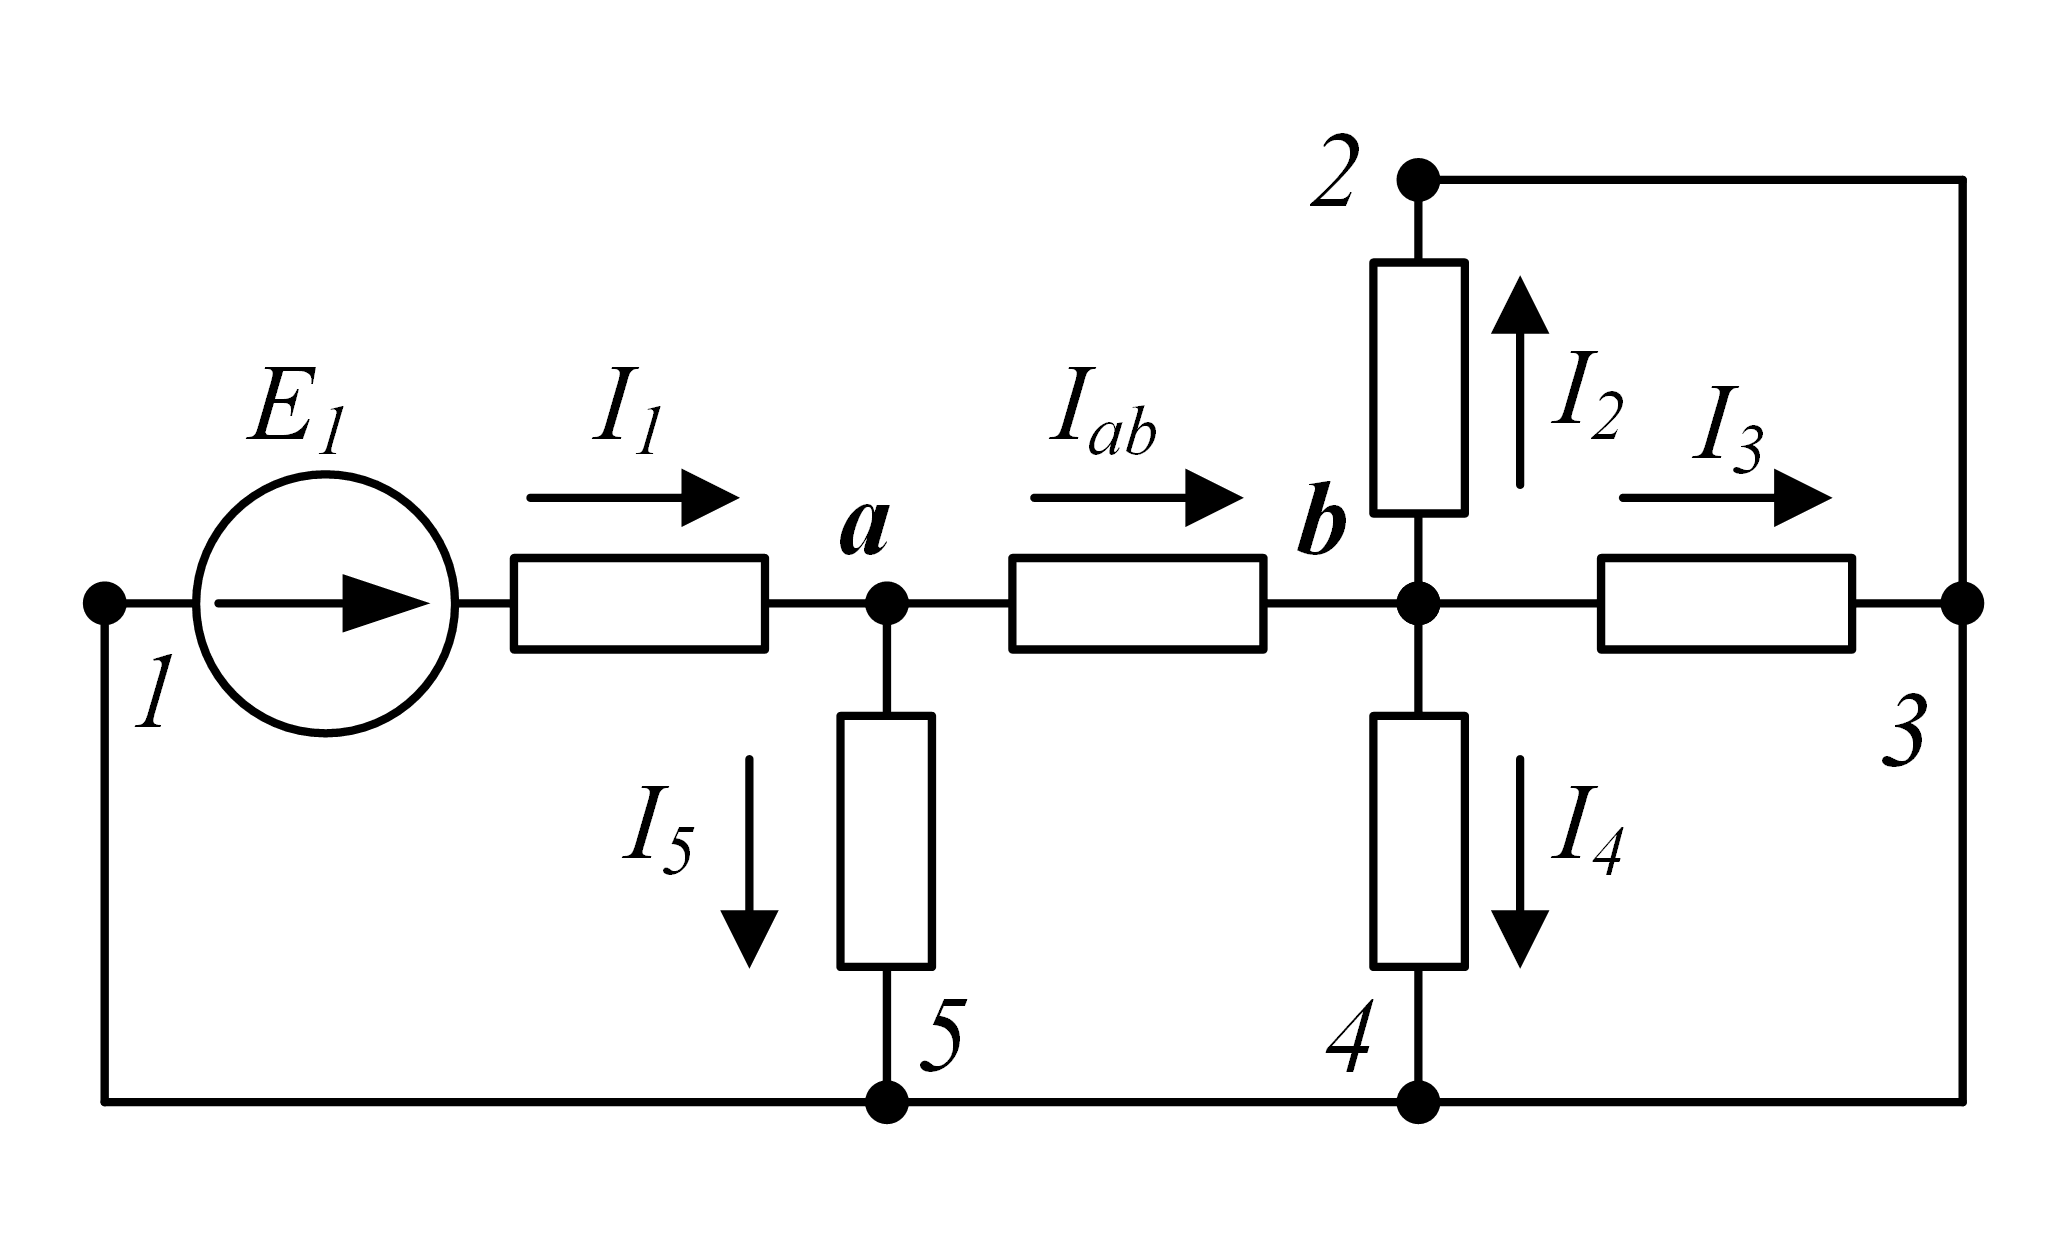
\includegraphics[width=1\linewidth]{pic/2-6_b}} \\ \textit{б)}
			\end{minipage}
			\vfill
			\begin{minipage}[]{0.4\linewidth}
				\center{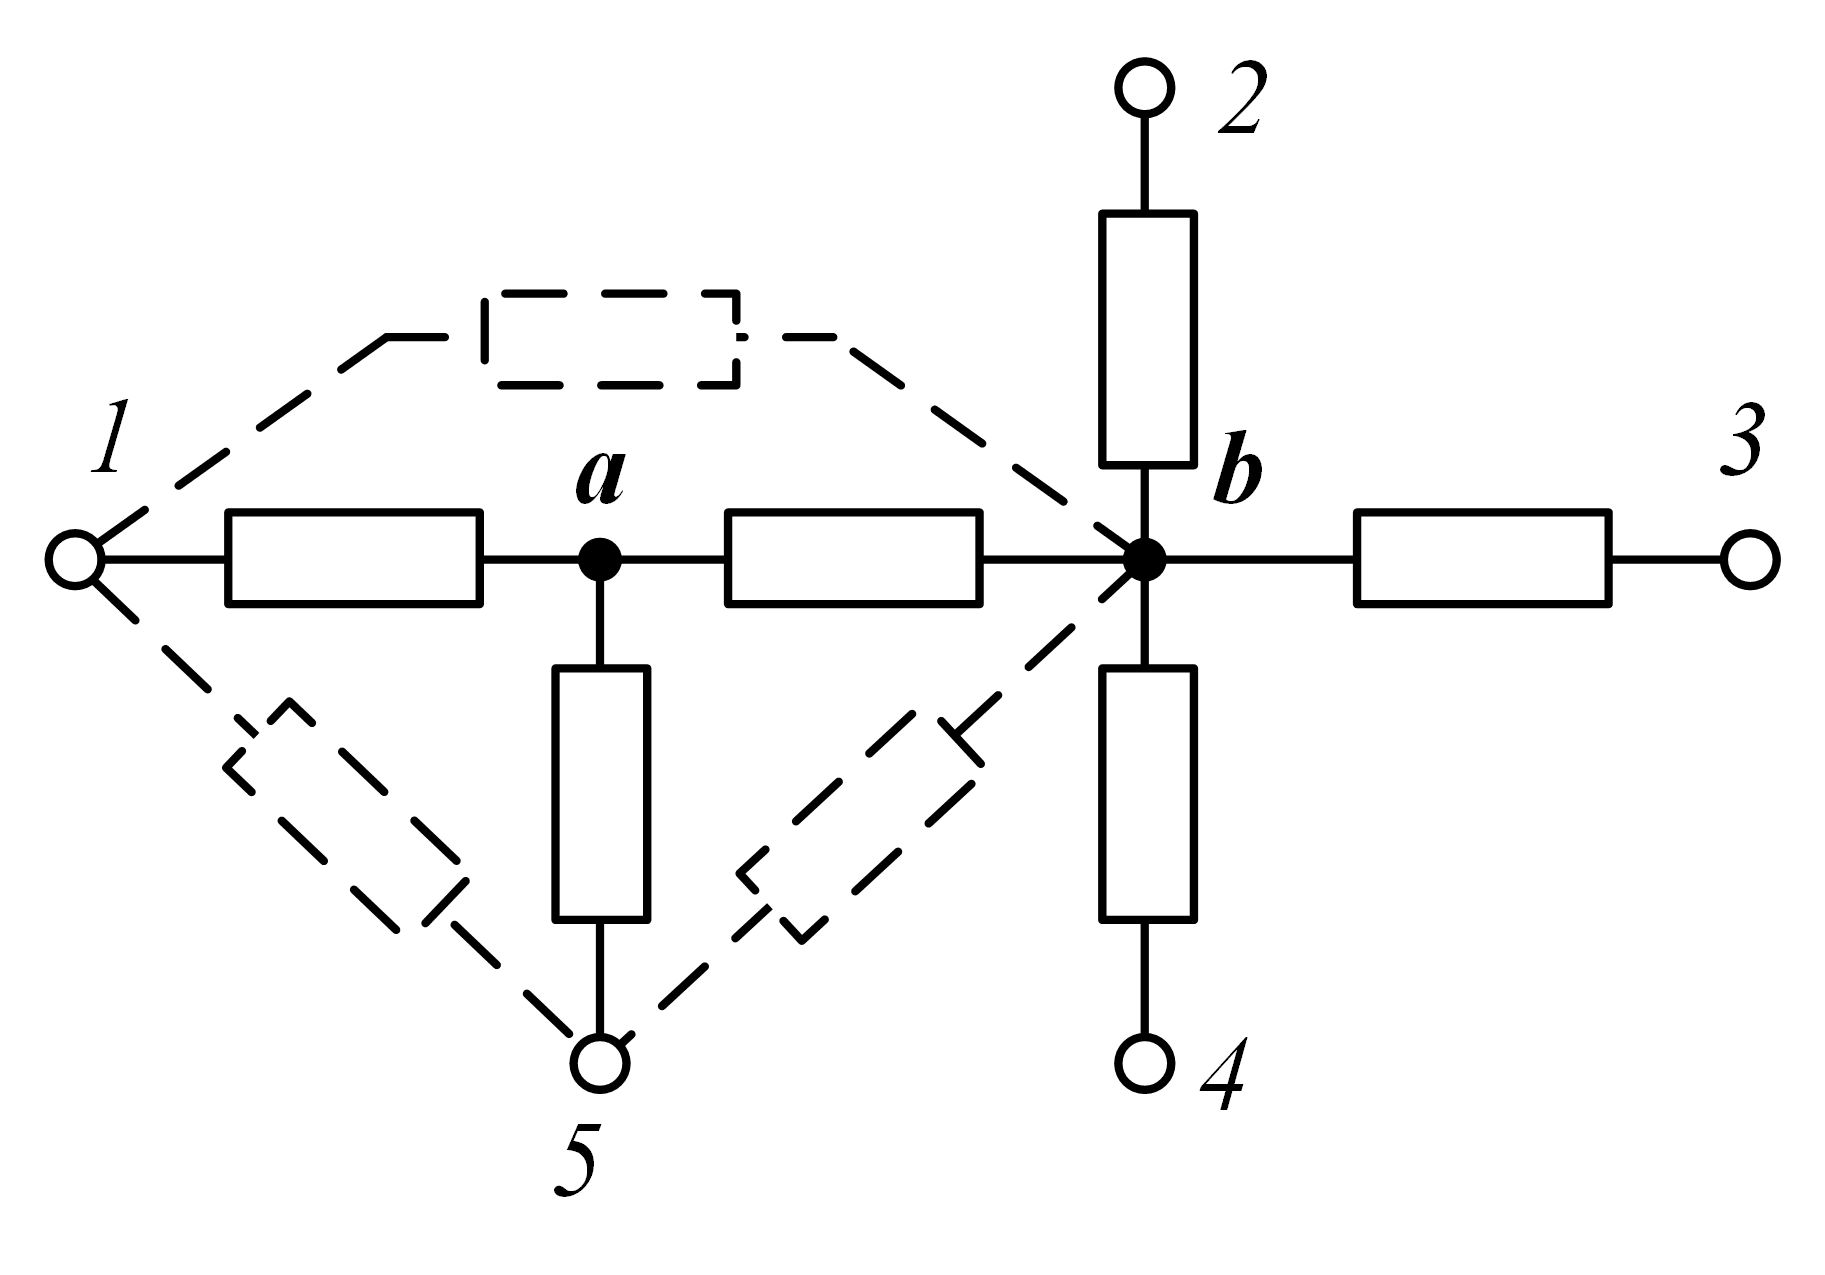
\includegraphics[width=1\linewidth]{pic/2-6_v}} \\ \textit{в)}
			\end{minipage}
			\hfill
			\begin{minipage}[]{0.47\linewidth}
				\center{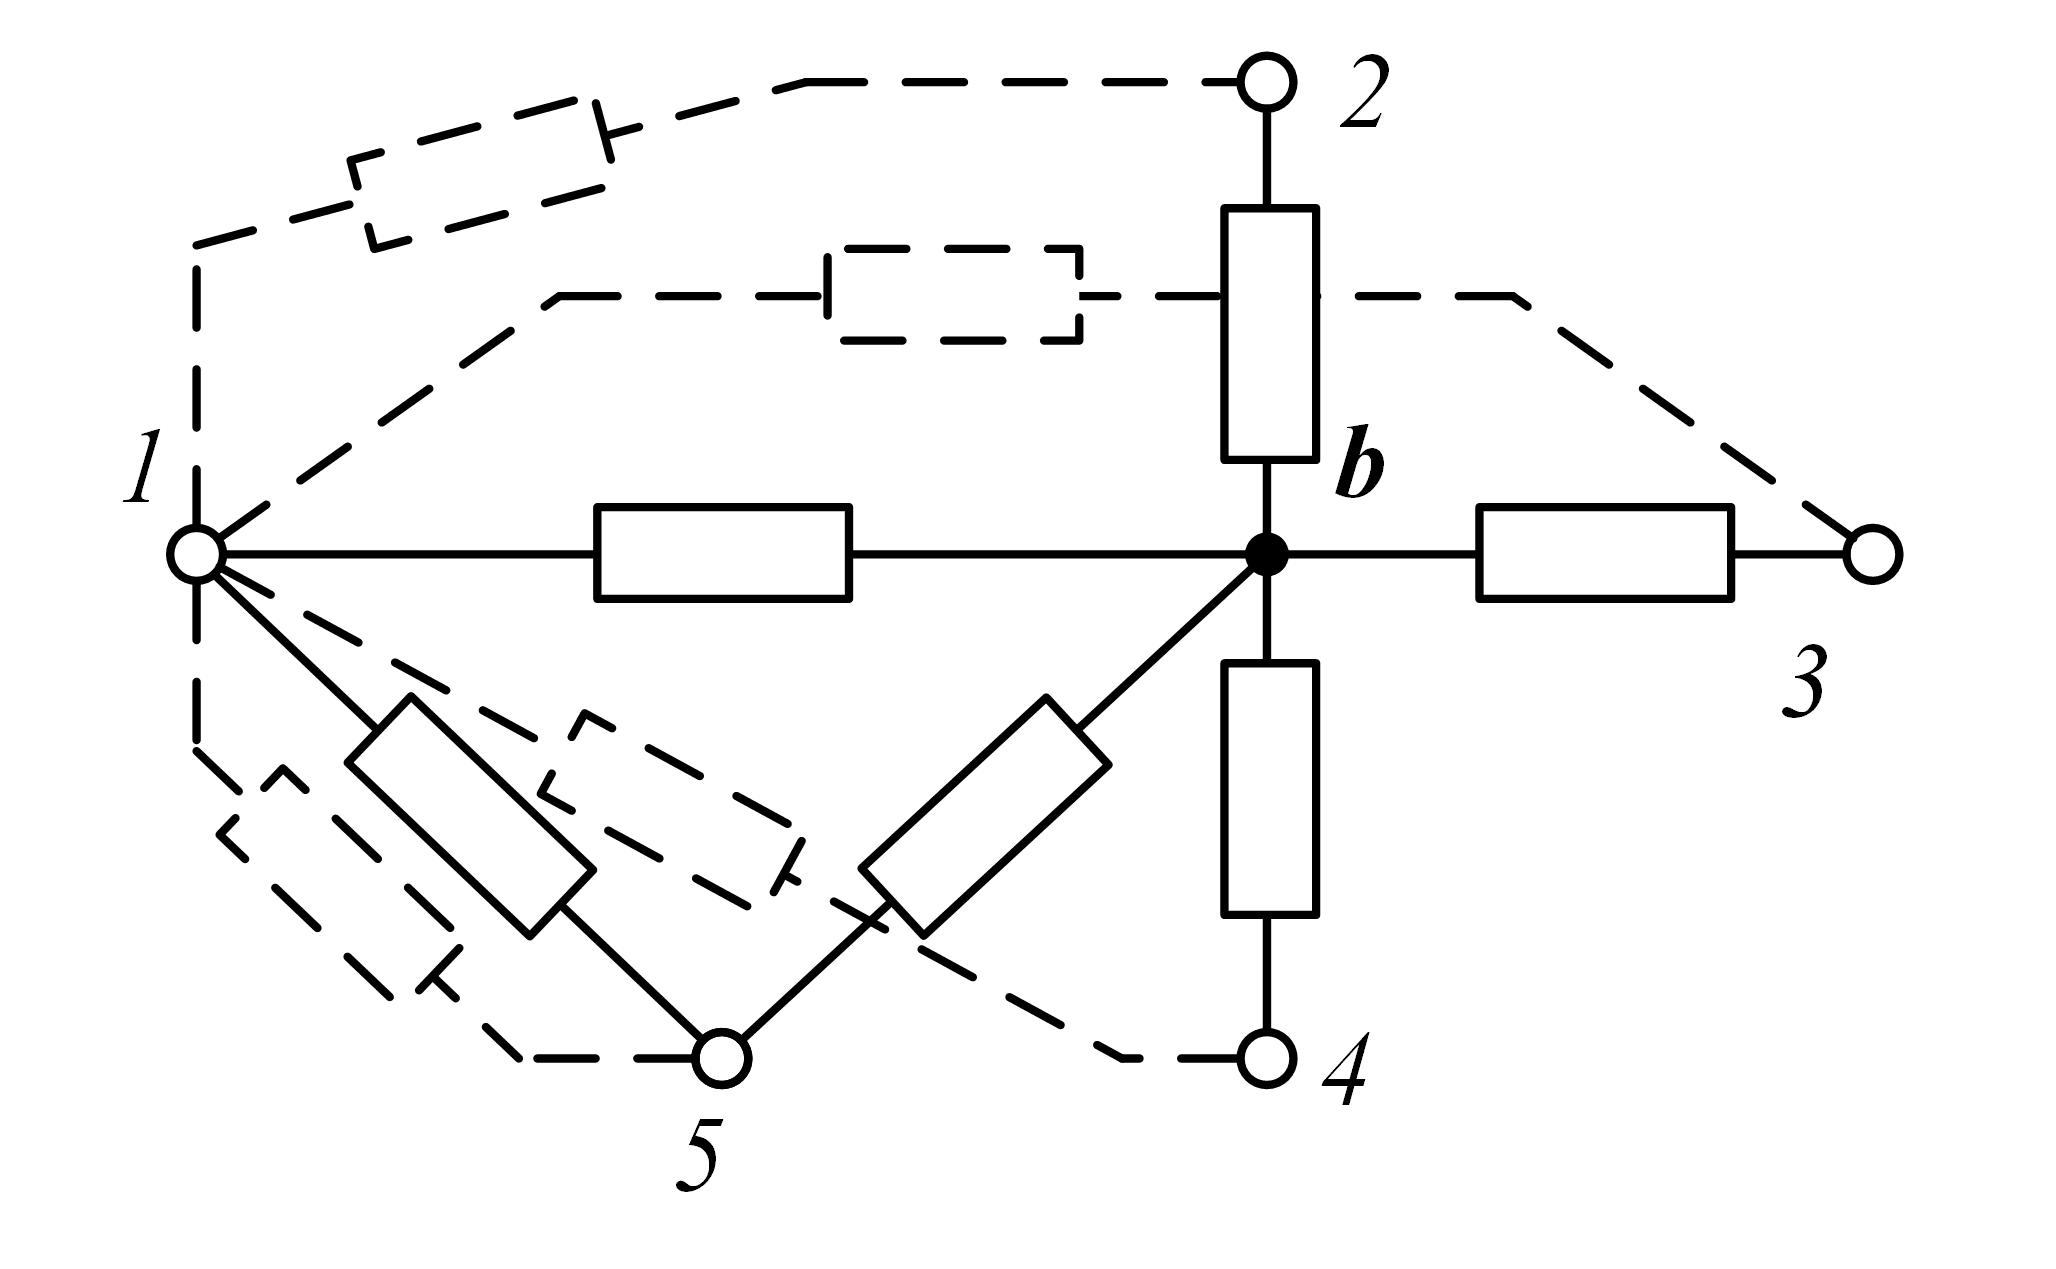
\includegraphics[width=1\linewidth]{pic/2-6_g}} \\ \textit{г)}
			\end{minipage}
			\caption{К примеру \ref*{chap:2 obshchie ukazaniia k vypolneniiu raschetov}-\arabic{example}: \textit{а} --- исходная схема; \textit{б} --- к применению способа токораспределения; \textit{в} и \textit{г} --- этапы преобразования схемы.}
			\label{ris:2-6 k_primeru_2-4}
		\end{figure}
		
		Искомые реактивности будут: $ x_{11} = 5,2 / 4,5 = 1,15 $; $ x_{12} = 5,2 / 0,86 = 6,05 $; $ x_{13} = 5,2 $; $ x_{14} = 5,2 / 1,9 = 2,74 $ и $ x_{15} = 5,2 / 0,74 = 7 $. Читатель может убедиться, что $ x_{12} // x_{13} // x_{14} // x_{15} = 6,05 // 5,2 // 2,74 // 7 = 1,15 = x_{11} $.
		
		\item Преобразуем звезду в треугольник с вершинами \textit{1}, \textit{b}, \textit{5} (рис.~\ref{ris:2-6 k_primeru_2-4},\textit{в}); $ x_{1b} = 0,4 + 0,5 + (0,4 \cdot 0,5/4,56) = 0,94 $; $ x'_{15} = 0,4 + 4,56 + (0,4 \cdot 4,56/0,5) = 8,61 $ и $ x_{5b} = 0,5 + 4,56 + (0,5 \cdot 4,56 / 0,4) = 10,76 $. Как видно из рис.~\ref{ris:2-6 k_primeru_2-4},\textit{г}, образовалась пятилучевая звезда с центром \textit{b}. Теперь, используя формулы преобразования многолучевой звезды в многоугольник (см. приложение~\colorbox{red}{П-1}), находим суммарную проводимость всех лучей звезды
		
		\begin{equation*}
			\sum Y = \frac{1}{0,94} + \frac{1}{1,74} + \frac{1}{1,5} + \frac{1}{0,79} + \frac{1}{10,76} = 3,66
		\end{equation*}
		
		и затем искомые реактивности:
		
		\begin{equation*}
			x_{12} = 0,94 \cdot 1,74 \cdot 3,66 = 6,05;
			\hspace{1pc}
			x_{13} = 0,94 \cdot 1,5 \cdot 3,66 = 5,2;
			\hspace{1pc}
			x_{14} = 0,94 \cdot 0,79 \cdot 3,66 = 2,74;			
		\end{equation*}
		
		при определении $ x_{15} $ должна быть учтена еще дополнительно параллельная ветвь $ x'_{15} = 8,61 $, т.~е.
		
		\begin{equation*}
			x_{15} = 0,94 \cdot 10,76 \cdot 3,66 // 8,61 = 7.
		\end{equation*}
		
		Разумеется результат тот же, что был получен выше.
		
		\item Определим сначала результирующую реактивность схемы относительно точки \textit{3}:
		
		\begin{equation*}
			x_7 = 0,4 // 4,56 = 0,37;
			\hspace{1pc}
			x_8 = 0,37 + 0,5 = 0,87;
		\end{equation*}
		\begin{equation*}
			x_9 = 0,87 // 1,74 // 0,79 = 0,335
			\hspace{1pc} и \hspace{1pc}
			x_{\sum} = 0,335 + 1,5 = 1,835.
		\end{equation*}
		
		Примем $ I_3 = C_3 = 1 $; тогда остальные коэффициенты распределения будут: $ C_2 = 1 \cdot 0,335 / 1,74 = 0,193 $; $ C_4 = 1 \cdot 0,335 / 0,79 = 0,424 $; $ C_1 + C_5 = 1 \cdot 0,335 / 0,87 = 0,338 $ (или $ 1 - 0,193 - 0,424 = 0,383 $); наконец, $ C_1 = 0,383 \cdot 0,37 / 0,4 = 0,354 $ и $ C_5 = 0,383 - 0,354 = 0,029 $. 
		
		Искомые взаимные реактивности найдем по (\ref{eq:2-37 Z_nK}), т.~е.
		
		\begin{equation*}
			x_{13} = \frac{1,835}{0,354} = 5,2 \text{~(то же значение, что и ранее);}
		\end{equation*}		
		\begin{equation*}
			x_{23} = \frac{1,835}{0,193} = 9,55;
			\hspace{1pc}
			x_{43} = \frac{1,835}{0,424} = 4,34;
			\hspace{1pc}
			x_{53} = \frac{1,835}{0,029} = 63,3.
		\end{equation*}
		
		Легко проверить, что те же взаимные реактивности получим, применяя предыдущие способы их определения. Так, например, $ x_{23} $ является стороной многоугольника между вершинами \textit{2} и \textit{3}, т.~е. $ x_{23} = 1,74 \cdot 1,5 \cdot 3,66 = 9,55 $ и т.~д.
	\end{enumerate}

\end{small}


\section{Мощность короткого замыкания}
\label{sec:2-7 moshchnost korotkogo zamykaniia}

Отключающую способность выключателя при номинальном его напряжении $ U_{\text{н}} $ характеризуют номинальным отключаемым током $ I_{\text{от.н}} $ или пропорциональной ему номинальной отключаемой мощностью:

\begin{equation*}
	S_{\text{от.н}} = \sqrt{3}U_{\text{н}}I_{\text{от.н}}.
\end{equation*}

Соответственно, когда проверка выключателя производится по отключаемой мощности, последняя должна быть сопоставлена с так называемой \so{мощностью короткого замыкания}, которая независимо от вида короткого замыкания условно определяется как

\begin{equation} % 2-38
	\label{eq:2-38 S_kz_v_moment_t}
	S_{\text{к}t} = \sqrt{3}U_{\text{н}}I_{\text{к}t},
\end{equation}

где $ I_{\text{к}t} $ --- ток короткого замыкания в момент $ t $ размыкания контактов выключателя; \\
$ U_{\text{н}} $ --- номинальное напряжение ступени, для которой найден ток короткого замыкания.

Имея в виду, что при одних и тех же базисных условиях численные значения относительных токов и мощностей короткого замыкания одинаковы:

%TODO: в скане на формуле черки, проверить
\begin{equation} % 2-39
	\label{eq:2-39 S_kz_baz_from_I_kz}
	\underset{*}{S}\!\,_{\text{к(б)}} = \underset{*}{I}\!\,_{\text{к(б)}},
\end{equation}

представляется возможным вести расчет непосредственно для мощностей короткого замыкания.

При этом во избежание ошибок при выборе или проверке выключателей нужно помнить, что отключаемая мощность выключателя в общем случае не постоянна, а зависит от напряжения, при котором он работает.


